\documentclass[10pt,a4paper]{article}
\usepackage[utf8x]{inputenc}
\usepackage{ucs}
\usepackage[german]{babel}
\usepackage[left=2.00cm, right=2.00cm, top=2.00cm, bottom=2.00cm]{geometry}
\renewcommand\familydefault{\sfdefault}

\title{Zusammenfassung - Regelungstechnik}
\author{}
\date{2019}

%costum layout
\setlength{\parindent}{0cm}
\usepackage{fancyhdr}
%\usepackage{xcolor}
\pagestyle{fancy}
\fancyhf{}
\fancyhead[L]{
	\strut\rlap{\color{cyan!50!blue}\rule[-\dp\strutbox]{\headwidth}{\headheight}}
	\textcolor {white} {Zusammenfassung: Regelungstechnik (kurz)}}
\fancyfoot[L]{
	\strut\rlap{\color{cyan!50!blue}\rule[-\dp\strutbox]{\headwidth}{\headheight}}
	\textcolor {white} {zuletzt aktualisiert: \today}}
\fancyhead[R]{\textcolor{white}{Sommersemester 2019}}
%\lfoot{}
\fancyfoot[R]{\textcolor{white} {\thepage}}
%\renewcommand{\footrulewidth}{1pt}

%math
\usepackage{amsmath}
\usepackage{amsfonts}
\usepackage{amssymb}
\usepackage{amstext}
\usepackage{mathtools}

%graphics
\usepackage{graphicx}
\usepackage{floatflt}
\usepackage{float}

%tabular
\usepackage{tabularx}
\usepackage[font=small,labelfont=small]{caption}
\usepackage{colortbl}
\usepackage[dvipsnames]{xcolor}
\renewcommand{\arraystretch}{1.5}
%\arrayrulecolor{white}

%tikz
\usepackage{tikz}
\usetikzlibrary{shapes, petri}
\tikzstyle{ell}=[ellipse,draw, yshift=-2mm]
\tikzstyle{rec} = [rectangle, draw]
\tikzstyle{dia} = [diamond, aspect=2, draw, yshift=-5mm]
\tikzstyle{cir} = [circle, draw, minimum size=3mm]
\tikzstyle{arrHV} = [to path={-| (\tikztotarget)}]
\tikzstyle{arrVH} = [to path={|- (\tikztotarget)}]
\tikzstyle{whileright} = [xshift=20mm, yshift=-3mm]
\tikzstyle{whileleft} = [xshift=-20mm, yshift=-3mm]
\tikzstyle{txtright} = [above, xshift=15mm]
\tikzstyle{txtleft} = [above, xshift=-15mm]
\tikzstyle{empty} = [coordinate]
\usetikzlibrary{positioning}

%listings
\usepackage{listings}
\lstdefinestyle{costum} {
	language=Bash,
	basicstyle=\footnotesize\ttfamily,
	keywordstyle=\bfseries\color{cyan!50!blue},
	commentstyle=\itshape\color{black!50},
	%identifierstyle=\color{blue},
	stringstyle=\color{green!50!black},
	morekeywords={returns, loop, each},
	escapeinside={\%*}{*)}
}
\lstset{style=costum}

%multicol
\usepackage{multicol}
%\setlength{\columnseprule}{0pt}
%\setlength{\columnsep}{20.0pt}



%custom title color
\usepackage{titlesec}
%\titleformat{\section}
%{\color{cyan!80!blue}\normalfont\Large\bfseries}
%{\color{black}\thesection}{1em}{}

%\titleformat{\subsubsection}
%{\color{blue!30!black!70}\normalfont\bfseries}
%{\color{black}\thesection}{1em}{}

\setcounter{secnumdepth}{4}

%\titleformat{\paragraph}
%{\color{green!30!black!70}\normalfont\normalsize\bfseries}{\theparagraph}{1em}{}
%\titlespacing*{\paragraph}
%{0pt}{3.25ex plus 1ex minus .2ex}{1.5ex plus .2ex}

%tab
\newcommand{\tab}[1][1]{\hspace*{#1cm}}

%color_summary
\newcommand{\sumcolor}[1]{\textcolor{red!10!green!40!blue}{#1}}

%coloring
\newcommand{\redr}{\textcolor{red}{r}}
\newcommand{\greeng}{\textcolor{green}{g}}
\newcommand{\blueb}{\textcolor{blue}{b}}

%vector
\newcommand{\vect}[1]{\ensuremath{\begin{bmatrix}#1\end{bmatrix}}}

%other
\usepackage{enumerate}
\usepackage{hyperref}
\usepackage{mathpartir}
\usepackage{trfsigns}
\usepackage{multicol}
\usepackage{ulem}
\usepackage{multirow}


%TODO
% Hinweise:
% -----
% Ruhelage
% Partialbruchzerlegung
%
% Fix:
% ---
% 2.1.1 Blockschaltbild P-Glieder

%checklist:
% section 1: y
% section 2: y ohne linearisierung am AP
% section 3: y ohne zustandsgleichungen mit stoergroesse
% section 4: y 
% section 5: y
% section 6: y
% section 7: y
% section 8: y
% section A: y
% section B: y
% section C: y
% section D: y




\begin{document}
	\tableofcontents
	\pagebreak
	
\section{Begriff der Regelung}
\subsection{Signale und Blöcke:}
\begin{tabularx}{\columnwidth}{llX}
	Bezeichnung & Var. & Beschreibung \\
	\hline
	Führungsgröße & $w(t)$ & Von außen vorgegebener Soll-Verlauf für die Regelgröße y(t) \\
	Regelgröße & $y(t)$ & Ausgangsgröße, der ein gewünschtes Verhalten aufgeprägt werden soll \\
	Regelabweichung & $e(t)$ & Entsteht durch Vergleich der Führungsgröße mit der gemessenen Regelgröße und soll klein gehalten werden ($e(t) = w(t) - y'(t)$) \\
	Stellgröße & $u(t)$ & Eingangsgröße, durch die das System gezielt beeinflusst werden kann \\
	Störgröße & $z(t)$ & Eingangsgröße, die störend und mit zumeist nur ungenau oder gar nicht bekannten Zeitverlauf auf das System wirkt \\
	Störgröße & $z_1(t)$ & Messbare Eingangsgröße, die störend auf das System wirkt \\
	Störgröße & $z_2(t)$ & Nicht-Messbare Eingangsgröße, die störend auf das System wirkt \\
	Messrauschen & $n(t)$ & \\
	Regler && Übertragungsglied, das aus der Regelabweichung das Stellsignal $u$ generiert, sodass $y$ möglichst $w$ folgt \\
	Messglied/Messeinrichtung && Erfasst die Regelgröße $y$ mittels eines Sensors und erzeugt ein zu $y(t)$ möglichst äquivalentes Signal $y'(t)$	\\
	Steuereinrichtung && Übertragungsglied, das den Stellgrößenverlauf $u(t)$ derart generiert, dass $y(t)$ einem vorgegebenen Sollverlauf $w(t)$ folgt. Besteht aus Störgrößenaufschaltung und Führungsgrößenaufschaltung \\
	Störgrößenaufschaltung && Übertragungspfad zur Aufschaltung einer messbaren Störgröße auf die Stellgröße \\
	Führungsgrößenaufschaltung && Übertragungspfad zur Aufschaltung der Führungsgröße auf die Stellgröße
\end{tabularx}

\subsection{Vorgeschaltete Steuereinrichtung}
\label{steuerung}
\subsubsection*{Blockschaltbild}
\begin{figure}[H]
	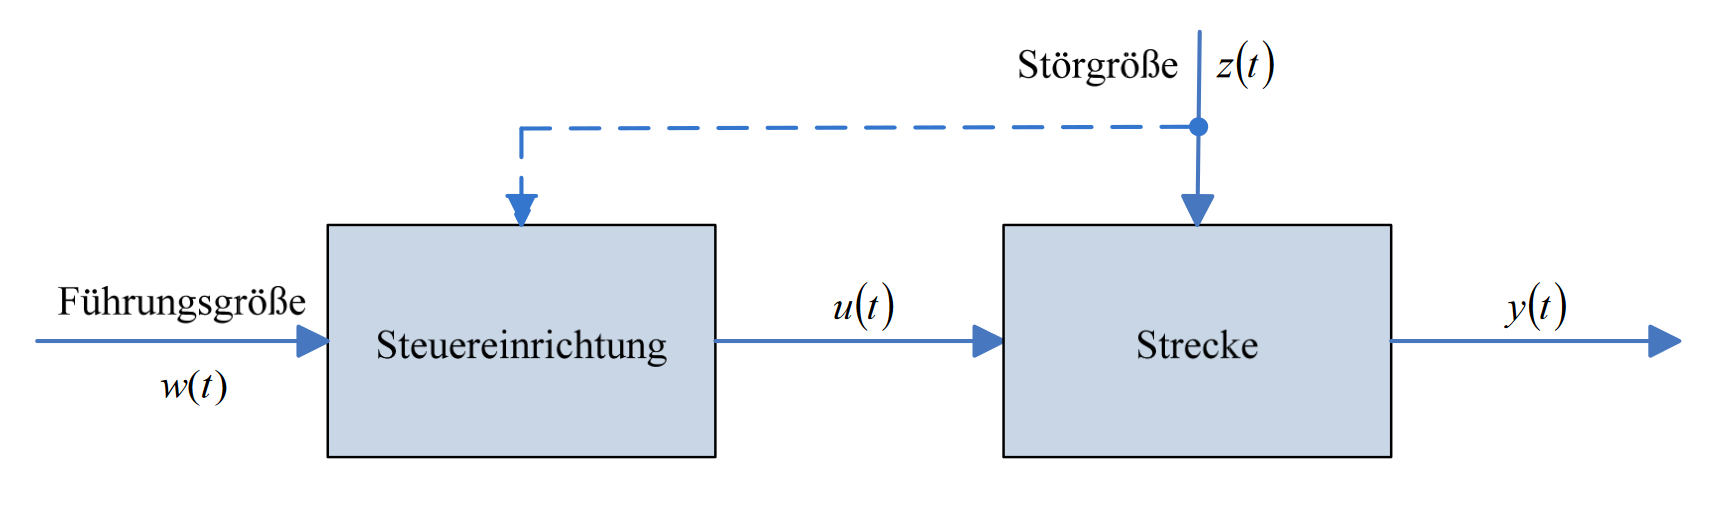
\includegraphics[width=0.6\columnwidth]{imgs/abb1_4.png}
\end{figure}

\subsection{Regelung}
\label{regelung}
\subsubsection*{Blockschaltbild}
\begin{figure}[H]
	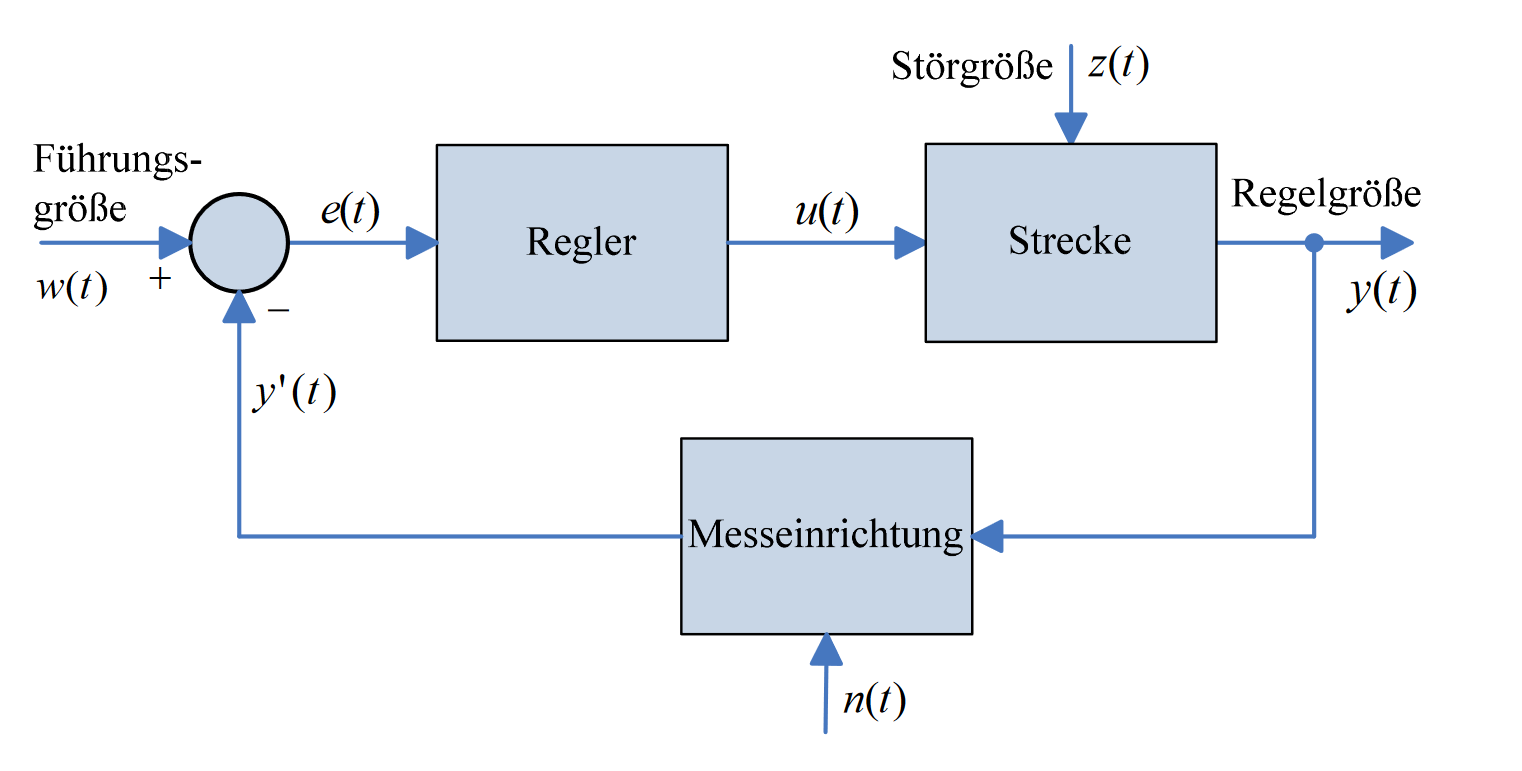
\includegraphics[width=0.6\columnwidth]{imgs/abb1_6.png}
\end{figure}

\subsection{Zwei-Freiheitsgrade-Regelung (Steuerung + Regelung)}
\subsubsection*{Blockschaltbild}
\begin{figure}[H]
	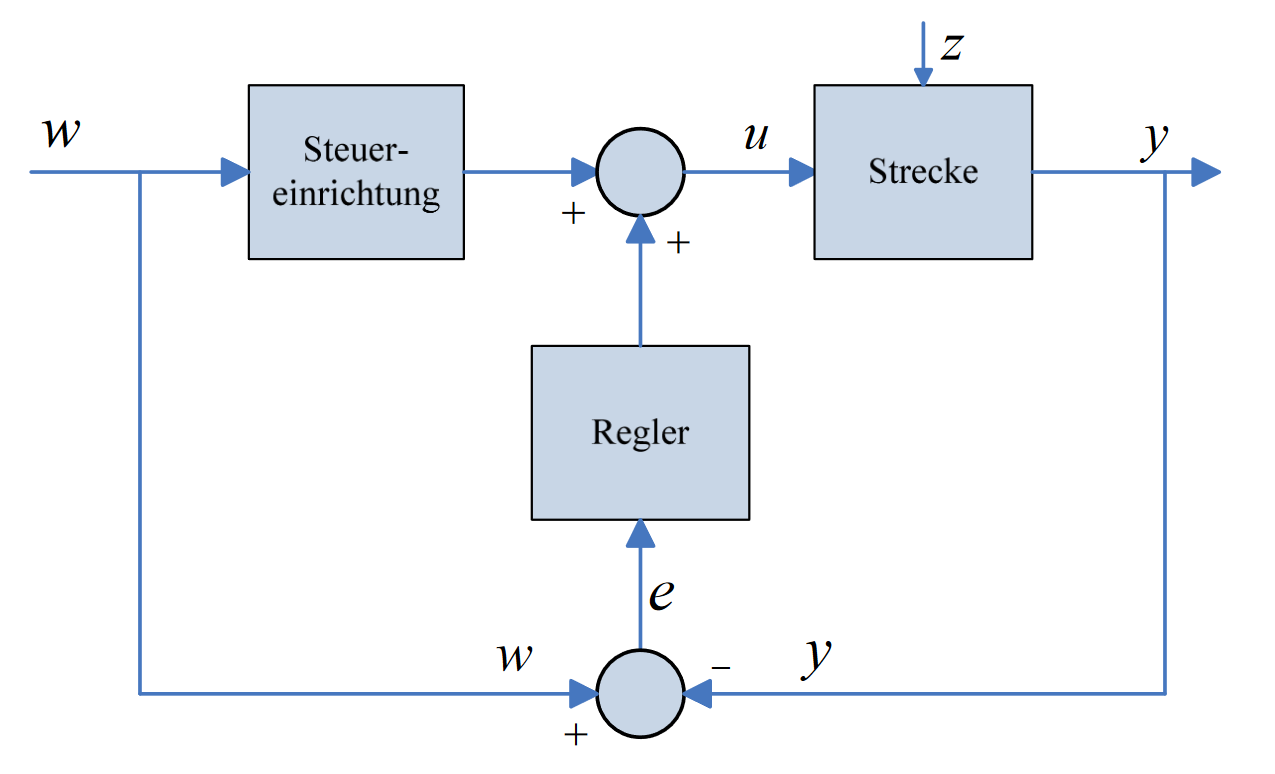
\includegraphics[width=0.6\columnwidth]{imgs/abb1_8.png}
\end{figure}

\subsubsection{Störgrößenaufschaltung}
\subsubsection*{Blockschaltbild}
\begin{figure}[H]
	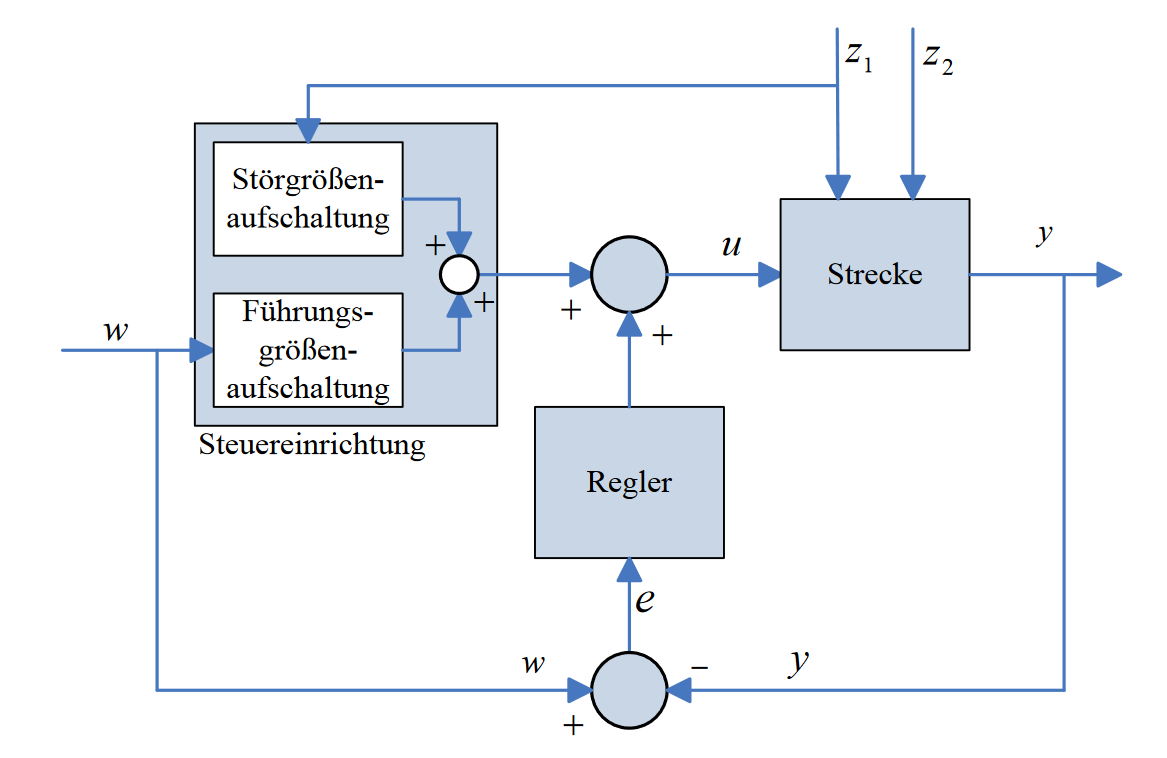
\includegraphics[width=0.6\columnwidth]{imgs/abb1_11.png}
\end{figure}

\section{Modelle}
\subsection{Zustandsdarstellung (bei Linearkombinationen)}
Bestehen die rechten Seiten der Zustandsgleichungen ausschließlich aus Linearkombinationen, d.h.:
$$
\begin{array}{l}
	\dot x_1 = a_{11} x_1 + \dots + a_{1n} x_n + e_1 z + b_1 u \\
	\tab \vdots \\
	\dot x_n = a_{n1} x_1 + \dots + a_{nn} x_n + e_n z + b_n u \\
	y = c_1 x_1 + \dots + c_n x_n
\end{array}	
$$
so gilt:
$$
\begin{array}{lcl}
	\dot{x} = A x + e z + b u & ≡ & \vect{\dot x_1 \\ \vdots \\ \dot x_n} = \vect{a_{11} & \dots & a_{1n} \\ \vdots & \ddots & \vdots \\ a_{n1} & \dots & a_{nn}} \vect{x_1 \\ \vdots \\ x_n} + \vect{e_1 \\ \vdots \\ \dot e_n} z + \vect{b_1 \\ \vdots \\ \dot b_n} u \\
	y = c^Tx & ≡ & y = \vect{c_1 & \dots & c_n} \vect{x_1 \\ \vdots \\ x_n}
\end{array}
$$

\paragraph*{Blockschaltbild:} ~\\
\begin{figure}[H]
	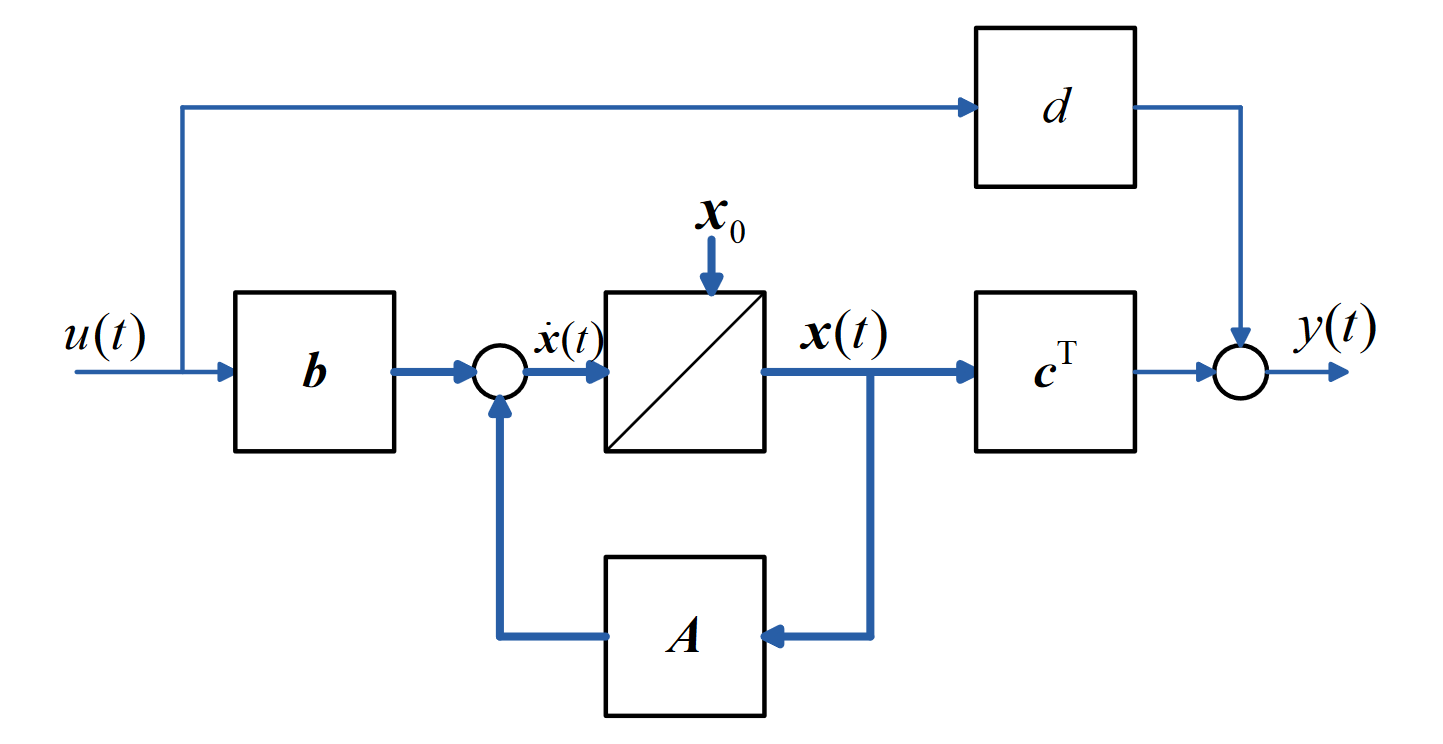
\includegraphics[width=0.6\columnwidth]{imgs/abb2_12.png}
\end{figure}

\subsection{Elementare Übertragungsglieder}
\textbf{Summationsglied:}
\begin{figure}[H]
	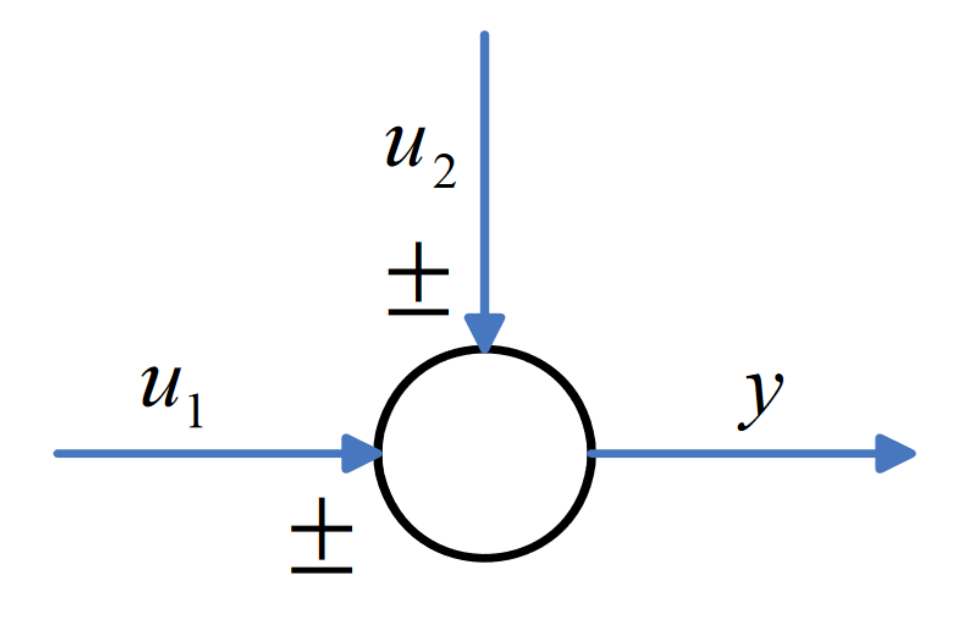
\includegraphics[width=0.2\columnwidth]{imgs/sumglied.png}
\end{figure}

\textbf{Weitere Übertragungsglieder:}
\begin{figure}[H]
	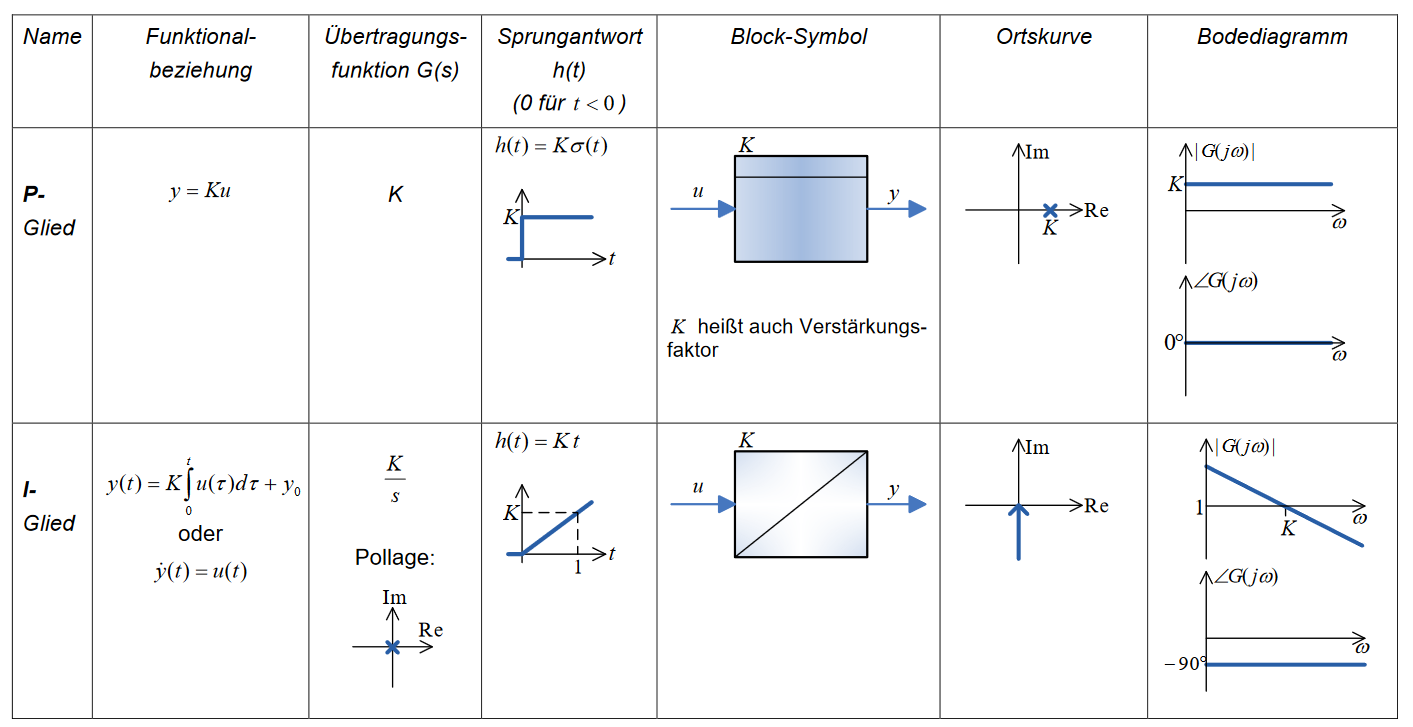
\includegraphics[width=1\columnwidth]{imgs/bb2_2a.png}
\end{figure}
\begin{figure}[H]
	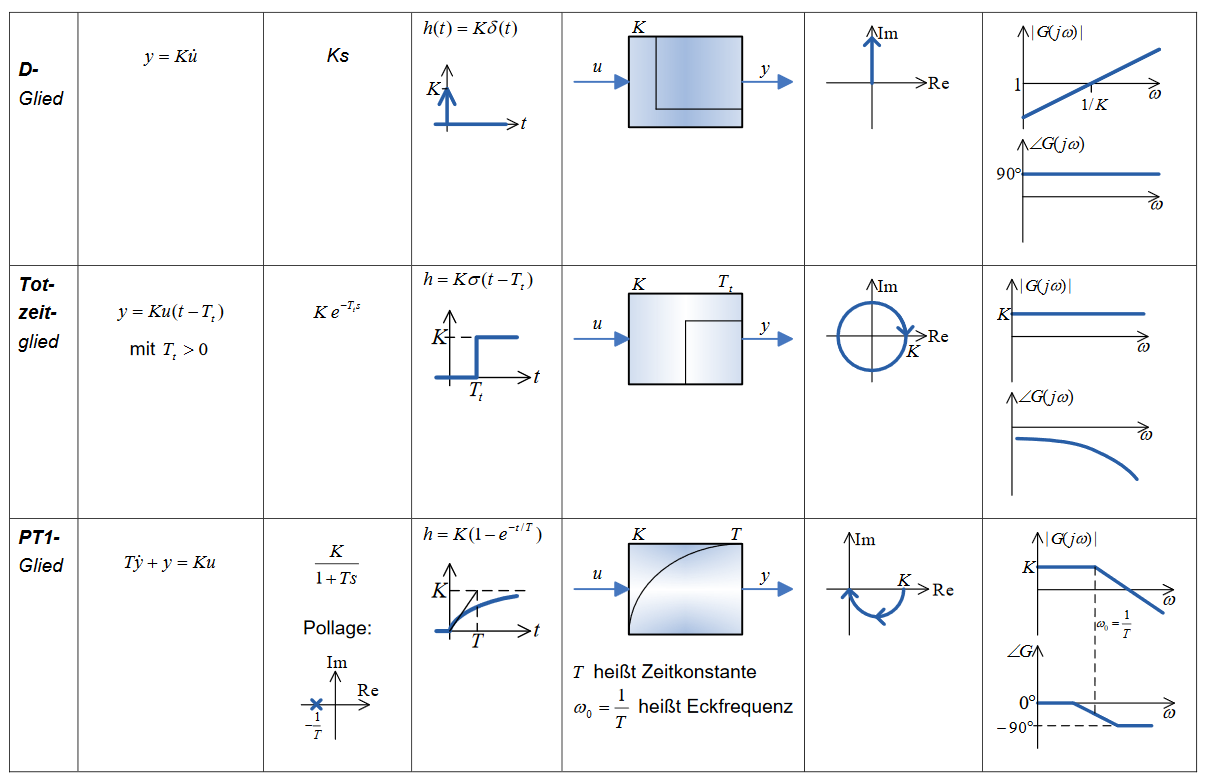
\includegraphics[width=1\columnwidth]{imgs/bb2_2b.png}
\end{figure}
\begin{figure}[H]
	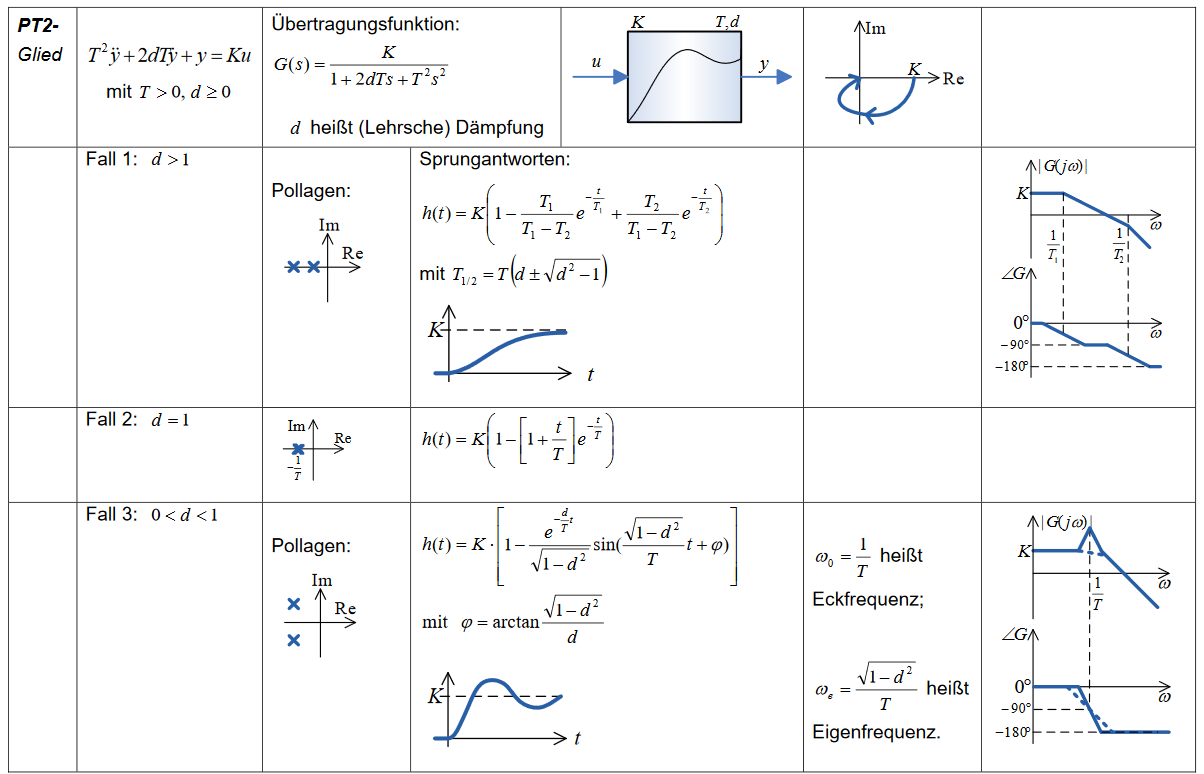
\includegraphics[width=1\columnwidth]{imgs/bb2_2c.png}
\end{figure}

\textbf{PT2-Glied (weitere Eigenschaften):} \\
\begin{itemize}
	\item Anfangssteigung der Sprungantwort $= 0$
	\item Eigenschaft der Lehrschen Dämpfung $d$:
	$$
		\begin{array}{ll}
		d > 1 & \text{aperiodischer Fall} \\
		d = 1 & \text{aperiodischer Grenzfall} \\
		0 < d < 1 & \text{aklingende Schwingung} \\
		d = 0 & \text{Dauerschwingung (instabil)} \\
		d < 0 & \text{aufklingende Schwingung (instabil)} \\
		
		\end{array}
	$$
\end{itemize}

\begin{figure}[H]
	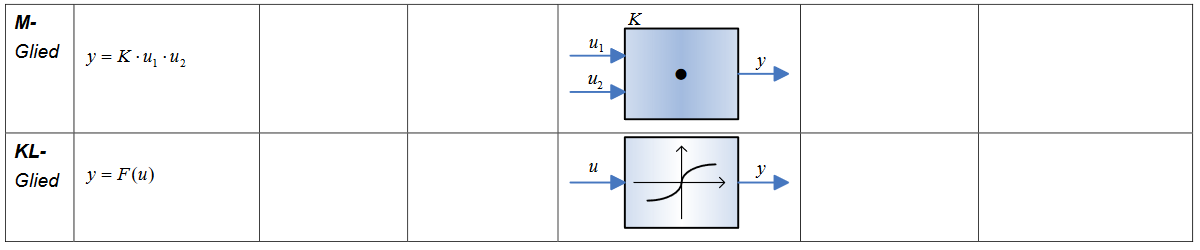
\includegraphics[width=1\columnwidth]{imgs/bb2_2d.png}
\end{figure}

Die Übertragungsglieder Summationsglied, Proportionalglied, Integrierglied, Differenzierglied und Totzeitglied sind linear.

\subsection{Lineare zeitinvariante Modelle (LZI-Modelle)}
\subsubsection{Regelungsnormalform}

Das System $y^{(n)} + a_{n-1} y^{(n-1)} + \dots + a_1 \dot y + a_0 y = b_{n-1} u^{n-1} + \dots + b_1 \dot u + b_0 u$ \\
besitzt die Zustandsdarstellung (Regelungsnormalform)
$$
\dot x = \begin{bmatrix}
0 & 1 & 0 & \dots & 0 \\
0 & 0 & 1 & \ddots & \vdots \\
\vdots & \vdots & \ddots & \ddots & 0 \\
0 & 0 & \dots & 0 & 1 \\
-a_0 & -a_1 & \dots & -a_{n-2} & -a_{n-1}
\end{bmatrix} x + \vect{0 \\ \vdots \\ \vdots \\ 0 \\ 1} u
$$
$$
y = \vect{b_0 & b_1 & \dots & b_{n-1}} x
$$

\subsubsection{Beobachtungsnormalform}
Das System $y^{(n)} + a_{n-1} y^{(n-1)} + \dots + a_1 \dot y + a_0 y = b_{n-1} u^{n-1} + \dots + b_1 \dot u + b_0 u$ \\
besitzt die Zustandsdarstellung (Beobachtungsnormalform)
$$
\dot x = \begin{bmatrix}
0 & 0 & \dots & 0 & -a_0 \\
1 & 0 & \ddots & 0 & -a_1 \\
0 & 1 & \ddots & 0 & -a_2\\
\vdots & \ddots & \ddots & 0 & \vdots \\
0 & \dots & 0 & 1 & -a_{n-1}
\end{bmatrix} x + \vect{b_0 \\ b_1 \\ b_2 \\ \vdots \\ b_{n-1}} u
$$
$$
y = \vect{0 & \dots & 0 & 1} x
$$


\subsection{Linearisierung im Arbeitspunkt}
\subsubsection{Mehere Eingabeparameter}
Sei $y = F(u_1, \dots u_n)$ eine Übertragungsfunktion ($n \in \mathbb{N}$). \\
Die linearisierte Funktion um den Arbeitspunkt $(u_{1,s}, \dots, u_{n,s})$ wird wie folgt berechnet:
$$
\Delta y = f(\Delta u_1, \dots, \Delta u_n, u_{1,s}, \dots, u_{n,s}) = \frac{\partial F(u_1, \dots u_n)}{\partial u_1}\Bigg|_\textrm{AP} ⋅ \Delta u_1 + \dots + \frac{\partial F(u_1, \dots u_n)}{\partial u_n}\Bigg|_\textrm{AP} ⋅ \Delta u_n
$$
$$
	\textrm{AP} ≡ u_1 = u_{1,s}, \dots, u_n = u_{n,s}
$$
mit
%$$
%	\Delta y = y - y_s
%$$
$$
	y_s = F(u_s)
$$
$$
	\Delta u_1 = u_1 - u_{1,s}, \dots, \Delta u_n = u_n - u_{n,s}
$$
Die um den Arbeitspunkt linearisierte Beziehung zwischen den absoluten Größen ist definiert als:
$$
y_{lin} = f(u_1, \dots, u_n, u_{1,s}, \dots, u_{n,s}) = \Delta y + y_s  \tab \text{(Ersetze $\Delta u_1$ durch $u_1 - u_{1,s}, \dots$)}
$$

\section{Laplace-Transformation}
\subsection{Definition}
Die Korrespondenz wird wie folgt dargestellt:
$$
	f(t) ~\laplace ~F(s)
$$

\pagebreak

\begin{multicols}{2}
\subsection{Korrespondenztabelle (in der Prüfung ausgehändigt)} 

\begin{tabularx}{\columnwidth}{|X|X|}
	\hline
	$f(t)$ & $F(s)$ \\
	\hline
	\hline
	$\delta(t)$ (Dirac-Impuls)& 1 \\
	\hline
	$\delta(t - t_0)$ & $e^{-t_0 s}$ \\
	\hline
	$\sigma(t)$ (Einheitssprung) & $\frac 1 s$ \\
	\hline
	$\sigma(t - t_0)$ & $\frac{e^{-t_0 s}}{s}$ \\
	\hline
	$t$ & $\frac{1}{s^2}$ \\
	\hline
	$\frac{t^n}{n!}, n \in \mathbb{N}_0$ & $\frac{1}{s^{n + 1}}$ \\
	\hline
	$e^{\alpha t}$ & $\frac{1}{s - \alpha}$ \\
	\hline
	$\frac 1 T e^{-\frac t T}$ & $\frac{1}{1 + Ts}$ \\
	\hline
	$te^{\alpha t}$ & $\frac{1}{(s - \alpha)^2}$ \\
	\hline
	$\frac{t}{T^2} e^{- \frac t T}$ & $\frac{1}{(1 + Ts)^2}$ \\
	\hline
%\end{tabularx}
%\begin{tabularx}{\columnwidth}{|X|X|}
	$\frac{t^n}{n!}e^{\alpha t}$ & $\frac{1}{(s - \alpha)^{n + 1}}$ \\
	\hline
	$1 - e^{\alpha t}$ & $\frac{-\alpha}{s(s - \alpha)}$ \\
	\hline
	$1 - e^{-\frac{t}{T}}$ & $\frac{1}{s(1 + Ts)}$ \\
	\hline
	$\sin \omega t$ & $\frac{\omega}{s^2 + \omega^2}$ \\
	\hline
	$\cos \omega t$ & $\frac{s}{s^2 + \omega^2}$ \\
	\hline
	$e^{-\delta t}\sin \omega t$ & $\frac{\omega}{(s + \delta)^2 + \omega^2}$ \\
	\hline
	$e^{-\delta t}\cos \omega t$ & $\frac{s + \delta}{(s + \delta)^2 + \omega^2}$ \\
	\hline
	$t \sin \omega t$ & $\frac{2 \omega s}{(s^2 + \omega^2)^2}$ \\
	\hline
	$t \cos \omega t$ & $\frac{s^2 - \omega^2}{(s^2 + \omega^2)^2}$ \\
	\hline	
\end{tabularx} \\
\\

wobei \\
$f(t) = 0$ für $t < 0$, \\
$T > 0, t_0 > 0, \omega > 0$ reell, \\
$\delta$ beliebig reell und \\
$\alpha$ beliebig komplex.
\end{multicols}

\subsection{Eigenschaften der Laplace-Transformation (in der Prüfung ausgehändigt)} 
\begin{tabularx}{\columnwidth}{|X|X|X|}
	\hline
	Eigenschaft & Operation im Zeitbereich & Operation im Bildbereich \\
	\hline
	\hline
	Linearität & $c_1f_1(t) + c_2f_2(t)$ & $c_1 F_1(s) + c_2 F_2(s)$ \\
	\hline
	Differenziation & $\dot f(t)$ & $sF(s) - f(0)$ \\
	& $\ddot f(t)$ & $s^2 F(s) - sf(0) - \dot f(0)$ \\
	& $f^{(n)}(t)$ & $s^n F(s) - \sum_{k=0}^{n-1} f^{(k)}(0) s^{n-k-1}$ \\
	\hline
	Integration & $\int_0^t f(\tau) ~d\tau$ & $\frac 1 s F(s)$ \\
	\hline
	Dämpfung & $f(t) ⋅ e^{\alpha t}$ & $F(s-\alpha)$ \\
	\hline
	Faltung & $f_1(t) * f_2(t)$ & $F_1(s) ⋅ F_2(s)$ \\
	\hline
	Zeitverschiebung & $f(t - t_0), t_0 > 0$ & $e^{-t_0 s}F(s)$ \\
	\hline
	Diffenrentiation der Bildfunktion & $(-1)^n t^n f(t)$ & $F^{(n)}(s), n \in \mathbb{N}$ \\
	\hline
	Skalierung der Zeitachse & $f(\alpha t), \alpha > 0$ & $\frac 1 \alpha F(\frac s \alpha)$ \\
	\hline
	Anfangswertsatz & \multicolumn{2}{X|}{$\lim_{t → +0} f(t) = \lim_{s → ∞} s F(s)$, sofern $\lim_{t → +0} f(t)$ existiert} \\
	\hline
	Endwertsatz & \multicolumn{2}{X|}{$\lim_{t → ∞} f(t) = \lim_{s → 0} sF(s)$, sofern $\lim_{t → ∞} f(t)$ existiert} \\
	\hline
\end{tabularx}

\subsection{Lösung linearer zeitinvarianter Differentialgleichungen mittels Laplace-Transformation}
Sei $a_ny^{(n)} + \dots + a_1 \dot y + a_0 y = b_m u^{(m)} + \dots + b_1 \dot u + b_0 u$ mit $m ≤ n$ und $a_n ≠ 0$ die systembeschreibende Differentialgleichung.
Die Lösung dieser DGL erfolgt durch die folgenden 5 Schritte:
\begin{enumerate}
	\item Transformation der DGL in den Bildbereich mittels Laplace-Transformation
	\item Auflösen nach $Y(s)$. Sind alle Anfangswerte gleich null, resultiert: \\
	$Y(s) = \frac{b_ms^m + \dots + b_1s + b_0}{a_ns^n + \dots + a_1s + a_0} ⋅ U(s) ≡ Y(s) = G(s) ⋅ U(s)$
	\item Einsetzen von $U(s) ~\Laplace ~u(t)$ in $Y(s) = G(s) ⋅ U(s)$
	\item Durchführung einer Partialbruchzerlegung von $Y(s)$
	\item Rücktransformation in den Zeitbereich $y(t) ~\laplace ~Y(s)$
\end{enumerate}

\subsubsection{Komplexe Übertragungsfunktion}
Sei $Y(s) = G(s)U(s)$ eine systembeschreibende Differentialgleichung im Bildbereich. \\
$G(s) = \frac{Y(s)}{U(s)}$ heißt komplexe Übertragungsfunktion. \\
Komplexe Übertragungsfunktionen der in Sektion \ref{darstell_gs} genannten Darstellungsformen heißen rationale Übertragungsfunktionen. Die zugehörigen Übertragungsglieder heißen rationale Übertragungsglieder, kurz R-Glieder.

\subsection{Lösung der Zustandsgleichung mittels Laplace-Transformation}
Sei ein LZI-System gegeben mit $\dot x = Ax + bu$ und $y = c^T x$. \\
Die Zustandsgleichungen im Bildbereich sind:
$$
	X(s) = \underbrace{(sI-A)^{-1} b U(s)}_{\text{Anregungsterm}} + \underbrace{(sI-A)^{-1} x(0)}_{\text{Anfangswertterm}} ~\Laplace ~x(t)
$$
$$
	Y(s) = \underbrace{c^T(sI-A)^{-1} b U(s)}_{\text{Anregungsterm}} + \underbrace{c^T (sI - A)^{-1} x(0)}_{\text{Anfangswertterm}} ~\Laplace ~y(t)
$$
Die komplexe Übertragungsfunktion $G(s)$ ist:
$$
	G(s) = c^T(sI - A)^{-1} b = \frac{c^T(\textrm{Adjunkte}(sI-A))b}{\det(sI-A)} = \frac{Z(s)}{N(s)}
$$

\subsubsection{Polstellen}
Jeder Pol von $G(s)$ ist Eigenwert von $A$. Ein Eigenwert von $A$ ist genau dann Pol von $G(s)$, wenn er sich nicht herauskürzt, d.h. nicht gleichzeitig Nullstelle von $Z(s)$ ist.

\section{Analyse dynamischer Systeme}
\subsection{Systemantworten}
\subsubsection{Impulsantwort}
Sei $Y(s) = G(s) U(s)$ ein lineares zeitinvariantes System mit der komplexen Übertragungsfunktion $G(s)$. \\
Die Impulsantwort dieses Systems ist:
$$
	Y(s) = G(s) ~\Laplace ~g(t)
$$
mit $u(t) = \delta(t) ~\laplace ~U(s) = 1$,

\subsubsection{Sprungantwort}
Sei $Y(s) = G(s) U(s)$ ein lineares zeitinvariantes System mit der komplexen Übertragungsfunktion $G(s)$. \\
Die Sprungantwort dieses Systems ist:
$$
	Y(s) = \frac{G(s)} s = H(s) ~\Laplace ~h(t) = \int_0^t g(\tau) ~d\tau
$$
mit $u(t) = \sigma(t) ~\laplace ~U(s) = 1/s$,

\subsubsection{Systemantwort mittels Faltung}
Sei ein lineares zeitinvariantes System gegeben mit Eingangssignal $u(t)$, Ausgangssignal $y(t)$ und der Übertragungsfunktion $g(t)$. \\
Das Ein-Ausgangsverhalten dieses Systems lässt sich durch die Faltungsoperation beschreiben:
$$
	y(t) = g(t) * u(t) = \int_0^t g(t - \tau) u(\tau) ~d \tau
$$

\subsubsection{Endwertsatz der Laplace-Transformation}
Sei $y(t)$ eine Zeitfunktion sowie $Y(s)$ deren Laplace-Transformierte und
\begin{itemize}
	\item $y(t → ∞)$ existiert oder
	\item das System ist übertragungsstabil und das Eingangssignal konvergiert
\end{itemize}
Es gilt:
$$
	y(t → ∞) = \lim_{s → 0} [sY(s)]
$$

Für die Sprungantwort gilt:
$$
h(t → ∞) = G(0), \tab \text{sofern alle Pole von $G(s)$ links der $j$-Achse sind}
$$

\subsection{Stabilität}
\subsubsection{Sprungantwortstabilität, Übertragungsstabilität}
\begin{itemize}
	\item Ein lineares zeitinvariantes System ist übertragungsstabil/sprungantwortstabil, falls
	$$
		h(t → ∞) = \int_0^∞ g(\tau) ~d \tau  = c < ∞
	$$
	wobei $h(t) = \int_0^t g(\tau) ~d \tau$ die Sprungantwort des Systems ist. \\
	\item Ein rationales Übertragungsglied (R-Glied) ist genau dann sprungantwortstabil, wenn alle Pole der Übertragungsfunktion $G(s)$ in der linken komplexen Halbebene liegen.
\end{itemize}

\subsubsection{Asymptotische Stabilität} %
Sei ein LZI-System gegeben mit $\dot x = Ax + bu$ und $y = c^T x$
\begin{itemize}
	\item Das Zustandsraummodell ist genau dann asymptotisch stabil, wenn alle Eigenwerte der Matrix $A$ in der linken komplexen Halbebene liegen.
	\item Asymptotische Stabilität $\implies$ Übertragungsstabilität
\end{itemize}

\subsection{Stationäre Verstärkung}
Sei $G(s) = \frac{Y(s)}{U(s)}$ die komplexe Übertragungsfunktion eines Systems und \\
sei dieses System stabil. \\
Außerdem werde dieses System mit einem Sprungsignal $u(t) = \kappa \sigma(t), \kappa ≠ 0$ angeregt. \\
Die stationäre Verstärkung von $G(s)$ ist definiert als:
$$
	\frac{\lim_{t → ∞} y(t)}{\lim_{t → ∞} u(t)}
$$
\subsection{Frequenzgang}
\subsubsection{Systemantwort auf harmonische Anregung}
Sei $Y(s) = G(s)U(s)$ die beschreibende Gleichung eines R-Gliedes, welches mit $u(t) = A\sin(\omega t)$ angeregt wird. \\
Die Antwort diese R-Gliedes ist:
$$
	y(t) = y_D(t) + y_G(t)
$$
mit dem Dauerschwingungsanteil
$$
	y_D(t) = A|G(j\omega)| \sin(\omega t + \angle G(j \omega))
$$ \\

Ist das System $G(s)$ stabil, so gilt für große $t$:
$$
	y(t) = y_D(t)
$$

\textbf{Größen:} \\
\begin{tabular}{ll}
	Frequenzgang des Systems: & $G(j \omega)$ \\
	Betrag des Frequenzgangs: & $|G(j \omega)|$ \\
	Phase des Frequenzgangs: & $\angle G(j \omega) = \arctan(-\omega T)$
\end{tabular} \\

wobei
$$
	G(j \omega) = |G(j \omega)| e^{j \angle G(j \omega)}
$$

\subsubsection{Frequenzgangortskurve und Bode-Diagramm}
\subsubsection{Konstruktion von Bode-Diagramm}
Sei die komplexe Übertragungsfunktion eines R-Gliedes als Produkt einfacher Glieder gegeben, d.h.:
$$
	G(s) = K ⋅ \frac{(s-q_1) ⋅ \dots ⋅ (s - q_m)}{(s - p_1) ⋅ \dots ⋅ (s - p_n)} = K ⋅ (s - q_1) ⋅ \dots ⋅ (s - q_m) ⋅ \frac{1}{s - p_1} ⋅ \dots ⋅ \frac{1}{s - p_n} = K ⋅ G_1 ⋅ \dots ⋅ G_m ⋅ G_{m+1} ⋅ \dots ⋅ G_{n + m}
$$

Die Betragskennlinie ist:
$$
	|G(j \omega)|_{dB} = 20 \log |G_1| + \dots + 20 \log |G_{n + m}|
$$

Die Phasenkennlinie ist:
$$
	\angle G(j \omega) = \angle G_1 + \dots + \angle G_{n + m}
$$

\subsubsection{Graphische Konstruktion von Bode-Diagramm (Kurzform)}
\begin{center}
	$\begin{array}{|l|c|c|c|c|c|c|c|c|c|}
	\hline
	\multicolumn{10}{|c|}{\text{Umrechnungstabelle}} \\
	\hline
	x & 0,01 & 0,1 & 0,32 & 0,5 & 1 & 2 & 3,2 & 10 & 100 \\
	\hline
	20 \log_{10}(x) & -40 & -20 & \approx -10 & \approx -6 & 0 & \approx 6 & \approx 10 & 20 & 40 \\
	\hline
	\end{array}$
\end{center} ~\\

1. Zeitkonstantenform:
$$
	G(j \omega) = K ⋅ \frac{(j \omega)^k}{(j \omega)^l} ⋅ \frac{(\tilde T_1 j \omega + 1) ⋅ \dots ⋅ (\tilde T_r j \omega + 1) ⋅ (\tilde T_{r+1}^2 (j \omega)^2 + 2\tilde d_{r+1} \tilde T_{r+1} j \omega + 1) ⋅ \dots ⋅ (\tilde T_m^2 (j \omega)^2 + 2\tilde d_m \tilde T_m j \omega + 1)}{(T_1 j \omega + 1) ⋅ \dots ⋅ (T_s j \omega + 1) ⋅ (T_{s+1}^2 (j \omega)^2 + 2 d_{s+1} T_{s+1} j \omega + 1) ⋅ \dots ⋅ (T_n^2 (j \omega)^2 + 2 d_n T_n j \omega + 1)}
$$

2. Eckfrequenzen:
$$
	\tilde \omega_i = \frac{1}{|\tilde T_i|}, \tab \eta_i = -\frac 1 {\tilde T_i} \text{ (falls einfache Nullstelle)}
$$
$$
	\omega_i = \frac{1}{|T_i|}, \tab p_i = -\frac 1 {T_i} \text{ (falls einfacher Pol)}
$$

3. Amplitudengang: \\
$$\begin{array}{ll}
	\text{Startwert:} & A(\omega_{min}) = 20 \log_{10} \left(\frac{\omega_{min}^k}{\omega_{min}^l} ⋅ |K| \right) \tab[1] [dB] \\
	\text{Anfangssteigung:} & A'(\omega_{min})  = (k - l) ⋅ \frac{20 dB}{Dekade}
\end{array}$$
\begin{center}
\begin{tabular}{|l|l|c|}
	\hline
	\multicolumn{3}{|c|}{Verlauf} \\
	\hline
	\multicolumn{2}{|l|}{} & $A'(\omega_i^+) = A'(\omega_i^-) + \dots$ \\
	\hline
	\multirow{2}{*}{Nullstelle} & einfach & $20 dB/Dekade$ \\
	\cline{2-3}
	& doppelt/konjugiert komplex & $40 dB/Dekade$ \\
	\hline
	\multirow{2}{*}{Pol} & einfach & $-20 dB/Dekade$ \\
	\cline{2-3}
	& doppelt/konjugiert komplex & $-40 dB/Dekade$ \\
	\hline
\end{tabular}
\end{center}

4. Phasengang:
\begin{center}
	\begin{tabular}{|l|c|}
		\hline
		\multicolumn{2}{|c|}{Startwert} \\
		\hline
		Verstärkungsfaktor & $\varphi(\omega_{min})$ \\
		\hline
		$K > 0$ & $0° + (k-l) ⋅ 90°$ \\
		\hline
		$K < 0$ & $-180° + (k-l) ⋅ 90°$ \\
		\hline
	\end{tabular}
\end{center}

\begin{center}
	\begin{tabular}{|l|l|l|c|}
		\hline
		\multicolumn{4}{|c|}{Grobverlauf} \\
		\hline
		\multicolumn{3}{|l|}{} & $\varphi(\omega_i^+) = \varphi(\omega_i^-) + \dots$ \\
		\hline
		\multirow{4}{*}{Nullstelle} & \multirow{2}{*}{einfach} & $\eta_i < 0$ & $90°$ \\
		\cline{3-4}
		& & $\eta_i > 0$ & $-90°$ \\
		\cline{2-4}
		& \multirow{2}{*}{doppelt/konjugiert komplex} & $\Re(\eta_{i/i+1}) ≤ 0$ & $+180°$ \\
		\cline{3-4}
		& & $\Re(\eta_{i/i+1}) > 0$ & $-180°$ \\
		\hline
		\multirow{4}{*}{Pol} & \multirow{2}{*}{einfach} & $p_i < 0$ & $-90°$ \\
		\cline{3-4}
		& & $p_i > 0$ & $90°$ \\
		\cline{2-4}
		& \multirow{2}{*}{doppelt/konjugiert komplex} & $\Re(p_{i/i+1}) ≤ 0$ & $-180°$ \\
		\cline{3-4}
		& & $\Re(p_{i/i+1}) > 0$ & $+180°$ \\
		\hline		
	\end{tabular}
\end{center}

\begin{center}
	\begin{tabular}{|c|c|c|c|c|}
		\hline
		\multicolumn{5}{|c|}{Feinverlauf} \\
		\hline
		Änderung von Grobverlauf & \multicolumn{2}{c|}{Änderung bei -1 Dekade} & \multicolumn{2}{c|}{Änderung bei +1 Dekade} \\
		$\varphi(\omega_i^+) = \varphi(\omega_i^-) + \dots $ & Pfeile & $\varphi'(\omega^+) = \varphi'(\omega^-) + \dots $ & Pfeile & $\varphi'(\omega^+) = \varphi'(\omega^-) + \dots$ \\
		\hline
		$x ⋅ 90°$ & $x ⋅ ↑$ & $ x ⋅ 45°$ & $x ⋅ ↓$ & $ -x ⋅ 45°$ \\
		\hline
		$-x ⋅ 90°$ & $x ⋅ ↓$ & $ -x ⋅ 45°$ & $x ⋅ ↑$ & $ x ⋅ 45°$ \\
		\hline
	\end{tabular}
\end{center}
	



\section{Regelkreis und Stabilität}
\subsection{Standardregelkreis}
Der Standardregelkreis ist definiert als:
\begin{figure}[H]
	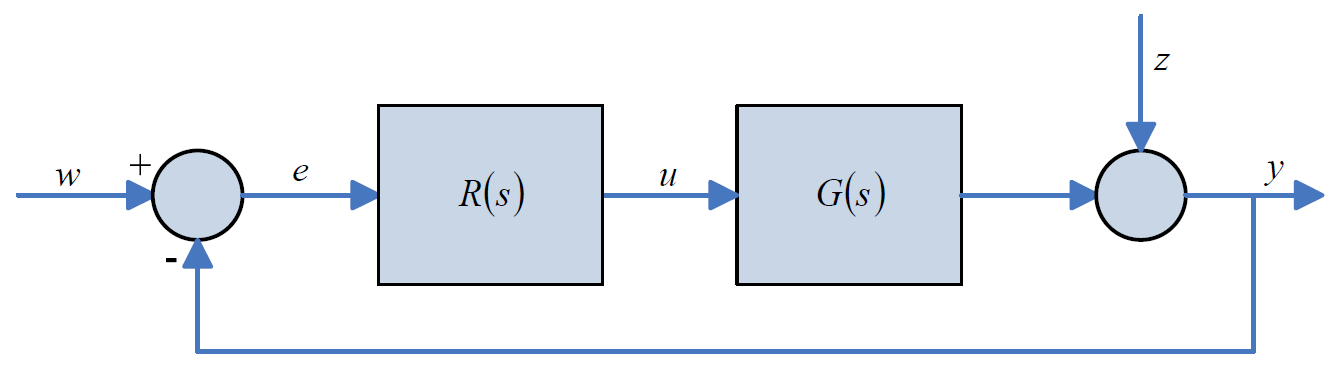
\includegraphics[width = \columnwidth]{imgs/standardregelkreis_2.png}
\end{figure}
mit dem Übertragungsverhalten:
$$
	Y(s) =\underbrace{ \frac{F_o(s)}{1 + F_o(s)}}_{\substack{T(s) \\ \text{Führungsübertra-} \\ \text{gungsfunktion}}} W(s) + \underbrace{\frac{1}{1 + F_o(s)}}_{\substack{S(s) \\ \text{Störübertragungs-} \\ \text{funktion}}} Z(s)
$$
wobei $F_o(s) = G(s)R(s)$ die Übertragungsfunktion des offenen Kreises ist.

\subsubsection{Führungsübertragungsfunktion $T(s)$}
Sei $F_o(s) = \frac{Z_o(s)}{N_o(s)}$ die Übertragungsfunktion des offenen Kreises des Standardregelkreises. \\
Die Führungsübertragungsfunktion des Standardregelkreises ist definiert als:
$$
	T(s) = \frac{F_o(s)}{1 + F_o(s)} = \frac{Z_o(s)}{Z_o(s) + N_o(s)}
$$

\subsubsection{Störübertragungsfunktion $S(s)$}
Sei $F_o(s) = \frac{Z_o(s)}{N_o(s)}$ die Übertragungsfunktion des offenen Kreises des Standardregelkreises. \\
Die Störübertragungsfunktion des Standardregelkreises ist definiert als:
$$
	S(s) = \frac{1}{1 + F_o(s)} = \frac{N_o(s)}{Z_o(s) + N_o(s)}
$$

\subsubsection{Eigenschaften des Standardregelkreises}
\subsection{Stabilität des Standardregelkreises}
\subsubsection{Übertragungsstabilität des Standardregelkreises}
Der Standardregelkreis ist genau dann übertragungsstabil bezüglich $S(s)$ und $T(s)$, wenn sämtliche Lösungen der charakteristischen Gleichung 
$$
	F_o(s) + 1 = 0
$$
in der linken komplexen Halbebene liegen.

\subsubsection{Asymptotische Stabilität des Standardregelkreises}
\textbf{Kriterium 1:} \\
Der Standardregelkreis ist genau dann asymptotisch stabil, wenn alle Lösungen der charakteristischen Gleichung 
$$
	Z_G(s)Z_R(s) + N_G(s)N_R(s) = 0
$$
in der linken  komplexen Halbebene liegen. Diese Lösungen sind die Systempole der Regelung. \\
Es gilt: 
$$
	G(s) = \frac{Z_G(s)}{N_G(s)}, \tab R(s) = \frac{Z_R(s)}{N_R(s)}
$$ \\

\textbf{Kriterium 2:} \\
Der Standardregelkreis ist genau dann asymptotisch stabil, wenn alle Lösungen der charakteristischen Gleichung
$$
	F_o(s) + 1 = 0
$$
in der linken komplexen Halbebene liegen und alle eventuelle Pol-Nullstellenkürzungen innerhalb der Strecke ($G(s)$), innerhalb des Reglers ($R(s)$) und zwischen Regler und Strecke ($G(s)R(s)$) ausschließlich links gelegene Pol-Nullstellenpaare betreffen.


\subsection{Nyquist-Kriterium}
\renewcommand{\arraystretch}{1}
\begin{tabular}{ll}
	$F_o(j \omega)$: & Frequenzgangortskurve des offenen Kreises des Standardregelkreises
\end{tabular}

\subsubsection{Voraussetzungen}
\begin{itemize}
	\item Allgemeines Nyquist-Kriterium
	\begin{enumerate}
		\item $F_o(s) = \frac{b_0 + b_1s + \dots + b_ms^m}{a_0 + a_1s + \dots + a_ns^n} ⋅ e^{-T_ts}$
		\item $m < n$ und $T_t ≥ 0$
	\end{enumerate}
	\item Einfaches Nyquist-Kriterium (zusätzlich)
	\begin{enumerate}
		\item Eines der folgenden Voraussetzungen ist erfüllt:
		\begin{enumerate}
			\item Alle Pole von $F_o(s)$ liegen in der linken komplexen Halbebene und $\frac{b_0}{a_0} > 0$
			\item Ein Pol liegt in null, alle anderen Pole von $F_o(s)$ liegen in der linken komplexen Halbebene und $\frac{b_0}{a_1} > 0$
			\item Zwei Pole liegen in null, alle anderen Pole von $F_o(s)$ liegen in der linken komplexen Halbebene und $\frac{b_0}{a_2} > 0$
		\end{enumerate}
	\end{enumerate}
	\item Einfaches Nyquist-Kriterium im Bode-Diagramm (zusätzlich)
	\begin{enumerate}
		\item Es gibt genau eine Durchtrittsfrequenz $\omega_c$ mit $|F_o(j \omega_c)| = 1 = 0 ~dB$. \\
	\end{enumerate}
\end{itemize}

\subsubsection{Allgemeines Nyquist-Kriterium}
\begin{tabular}{ll}
	$r_0$: & Anzahl der in der rechten komplexen Halbebene liegende Pole von $F_o(s)$ \\
	$a_0$: & Anzahl der auf der imaginären Achse gelegenen Pole von $F_o(s)$ \\
\end{tabular}
er Regelkreis ist genau dann übertragungsstabil, wenn die Winkeländerung $\omega_+$ des Fahrstrahls vom Punkt $-1$ zur Ortskurve
$$
	\omega_+ = r_0 \pi + a_0 \frac{\pi}{2}
$$
beträgt, während die Nyquist-Ortskurve $F_o(j \omega)$ von $\omega = 0$ bis $\omega = ∞$ durchlaufen wird. \\

\subsubsection{Einfaches Nyquist-Kriterium}
Liegt der Punkt $-1$ links der von der in Richtung wachsender $\omega$ durchlaufenden Frequenzgangortskurve $F_o(j \omega)$, so ist der Regelkreis übertragungsstabil. \\

\subsubsection{Einfaches Nyquist-Kriterium im Bode-Diagramm}
\begin{figure}[H]
	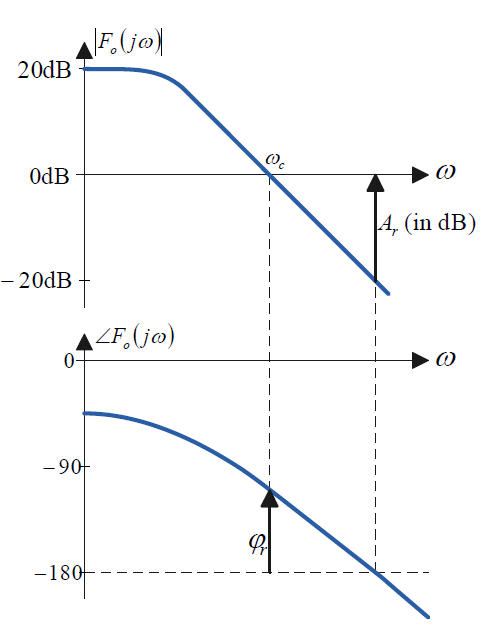
\includegraphics[width = 0.4\columnwidth]{imgs/nyquist_bode.png}
\end{figure}
Der Regelkreis ist übertragungsstabil, wenn
$$
	-180° < \angle F_o(j \omega_c) < 0
$$

\paragraph{Phasenreserve} ~\\
Die Phasenreserve $\varphi_r$ ist definiert als:
$$
	\varphi_r = \angle F_o(j \omega_c) + \pi
$$ \\

Ist $\varphi_r > 0$, so ist der Regelkreis übertragungsstabil.

\paragraph{Amplitudenreserve} ~\\
Sei $\omega_a$ die Frequenz, bei der der Phasengang gleich $-180°$ ist, d.h. $\angle F_o(j \omega_a) = -180°$ \\
Die Amplitudenreserver ist definiert als:
$$
	A_r = -|F_o(j \omega_a)|
$$ \\

Ist $A_r > 1$, so ist der Regelkreis stabil

\paragraph{Amplituden- und Phasenreserve in der Frequenzgangortskurve} ~\\
\begin{figure}[H]
	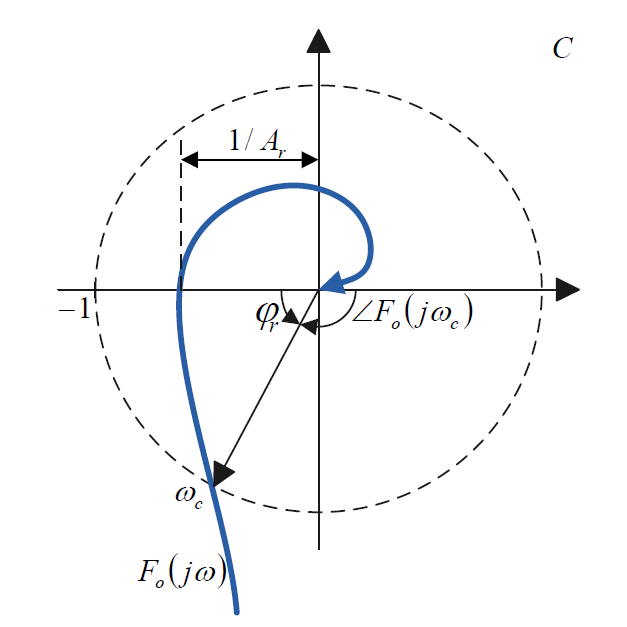
\includegraphics[width = 0.4\columnwidth]{imgs/nyquist_ortskurve.png}
\end{figure}

\subsection{Robustheit der Stabilität}
$\varphi_r$ und $A_r$ werden häufig als Maße der Robustheit der Stabilität gegenüber Fehlern oder Veränderungen des Modells $F_o(s)$ verwendet. Faustregel für gute Robustheit:
$$
	\varphi_r > 60° \tab \text{und/oder} \tab A_r > 2
$$ \\

\renewcommand{\arraystretch}{1.5}
\section{Reglerentwurf}
\subsection{Anforderungen an das Regelverhalten}
\begin{itemize}
	\item Dynamisches Verhalten:
	\item Stationäre Genauigkeit:
	\item Robuste Stabilität:
	\item Realisierbarkeit des Reglers:
	\item Einhaltung von Begrenzungen:
\end{itemize}

\subsection{Dynamik, Robustheit der Stabilität und Grenzen der Regelgüte}
\subsubsection{Bode-Theorem}
Sei der geschlossene Regelkreis übertragungsstabil, \\
sei Zählergrad von $F_o(s) + 2 ≤ $ Nennergrad von $F_o(s)$ und \\
sei $p_i$ die in der rechten komplexen Halbebene liegende Pole von $F_o(s)$ \\
Es folgt:
$$
	\int_0^∞ \ln|S(j \omega)| ~d \omega = 
	\begin{cases}
		0, & \text{sofern $F_o(s)$ stabil} \\
		\pi \sum_i  \Re(p_i), & \text{sofern $F_o(s)$ instabil}
	\end{cases}
$$

\subsection{Stationäre Genauigkeit}
\subsubsection{Stationäre Genauigkeit bezüglich des Führungsverhalten}
Ein Regelkreis ist stationär genau bezüglich des Führungsverhaltens genau dann, wenn
\begin{itemize}
	\item der geschlossene Regelkreis stabil ist
	\item und eine der folgenden (äquivalenten) Voraussetzungen erfüllt ist:
	\begin{itemize}
		\item Ein freies I-Glied ist im offenen Kreis vorhanden
		\item Die Übertragungsfunktion des offenen Kreises besitzt einen Pol im Ursprung
		\item Die Führungsübertragungsfunktion des geschlossenen Regelkreises hat eine stationäre Verstärkung von $1$
	\end{itemize}	
\end{itemize}

Es folgt:
$$
	\lim_{t → ∞} e(t) = 0 \text{ bzw. } \lim_{t → ∞} y(t) = \kappa, \tab \text{wobei } w(t) = \kappa \sigma(t), \kappa ≠ 0
$$

\subsubsection{Stationäre Genauigkeit bezüglich des Störverhaltens}
Ein Regelkreis ist stationär genau bezüglich des Führungsverhaltens genau dann, wenn
\begin{itemize}
	\item stationär genau bezüglich des Führungsverhalten ist
	\item und eine der folgenden (äquivalenten) Voraussetzungen erfüllt ist:
	\begin{itemize}
		\item Ein freies I-Glied ist im offenen Kreis zwischen Soll-/Istwert-Vergleich und Störeingriff vorhanden
		\item Die Störübertragungsfunktion des geschlossenen Regelkreises besitzt eine Nullstelle im Ursprung
		\item Die Störübertragungsfunktion des geschlossenen Regelkreises hat eine stationäre Verstärkung von $0$
	\end{itemize}	
\end{itemize}

Es folgt:
$$
	\lim_{t → ∞} e(t) = 0 \text{ bzw. } \lim_{t → ∞} y(t) = \kappa, \tab \text{wobei } w(t) = \kappa \sigma(t), \kappa ≠ 0 \text{ und } z(t) = \zeta \sigma(t), \zeta ≠ 0
$$

\subsection{Grundtypen linearer Regler}
Sei im folgenden die Regelabweichung $e(t)$ die Eingangsgröße der Regler und die Stellgröße $u(t)$ die Ausgangsgröße der Regler im Zeitbereich bzw. \\
$R(s)$ die komplexe Übertragungsfunktion des Reglers.

\subsubsection{P-Regler}
\textbf{Definition:}
$$
	\begin{array}{ll}
	\text{Zeitbereich:} & u(t) = K_R e(t) \\
	\text{Bildbereich:} & R(s) = K_R
	\end{array}
$$ \\

\textbf{Wahl der Variablen:} \\
$K_R:$ wird so gewählt, dass Phasen- und Amplitudenreserve groß genug sind, z.B: $A_r > 2, \varphi_r > 60°$ \\

\textbf{Vorteile/Nachteile:}
\begin{itemize}
	\item Vorteile:
	\begin{itemize}
		\item gute Dynamik bei einfachem Regleraufbau
	\end{itemize}
	\item Nachteile:
	\begin{itemize}
		\item keine stationäre Genauigkeit (außer wenn $G(s)$ ein I-Glied enthält und die Störung erst hinter dem I-Glied eingreift)
	\end{itemize}
\end{itemize}

\subsubsection{I-Regler}
\textbf{Definition:}
$$
	\begin{array}{ll}
	\text{Zeitbereich:} & u(t) = K_I \int_0^t e(\tau) ~d\tau \\
	\text{Bildbereich:} & R(s) = \frac{K_I}{s}
	\end{array}
$$ \\

\textbf{Wahl der Variablen:} \\
$K_I:$ wird so gewählt, dass Phasen- und Amplitudenreserve groß genug sind, z.B: $A_r > 2, \varphi_r > 60°$ \\

\textbf{Vorteile/Nachteile:}
\begin{itemize}
	\item Vorteile:
	\begin{itemize}
		\item sichert stationäre Genauigkeit
	\end{itemize}
	\item Nachteile:
	\begin{itemize}
		\item tendenziell langsame Dynamik der Regelung
	\end{itemize}
\end{itemize}

\subsubsection{PI-Regler}
\textbf{Definition:}
$$
	\begin{array}{ll}
	\text{Zeitbereich:} & u(t) = K_R e(t) + K_I \int_0^t e(\tau) ~d\tau \\
	\text{Bildbereich:} & R(s) = \frac{K_I}{s} (1 + T_R s) = \frac{K_I}{s} + K_R
	\end{array}
$$ \\

\textbf{Wahl der Variablen:} \\
$K_R = K_I ⋅ T_R$ \\
$T_R =$ größte Nennerzeitkonstante der Strecke (Zeitkonstantenform) \\
$K_I:$ wird so gewählt, dass Phasen- und Amplitudenreserve groß genug sind, z.B: $A_r > 2, \varphi_r > 60°$ \\

\textbf{Vorteile/Nachteile:}
\begin{itemize}
	\item Vorteile:
	\begin{itemize}
		\item schneller als I-Regler
		\item gesicherte stationäre Genauigkeit
	\end{itemize}
%	\item Nachteile:
%	\begin{itemize}
%		\item 
%	\end{itemize}
\end{itemize}


\subsubsection{PD-Regler}
\textbf{Definition:}
$$
	\begin{array}{ll}
	\text{Zeitbereich (ideal):} & u(t) = K_R (e(t) + T_R \dot e(t)) = K_R e(t) + K_D \dot e(t) \\
	\text{Bildbereich (ideal):} & R(s) = K_R(1 + T_R s) \\
	\text{Bildbereich (real):} & R(s) = K_R \frac{1 + T_R s}{1 + T_N s}, \tab T_N < T_R
	\end{array}
$$ \\

\textbf{Wahl der Variablen:} \\
$T_R=$ größte Streckenzeitkonstante  \\
$K_R:$ wird so gewählt, dass Phasen- und Amplitudenreserve groß genug sind, z.B: $A_r > 2, \varphi_r > 60°$ \\
$T_N: \frac{T_R}{50} < T_N < \frac{T_R}{5}$ \\

\textbf{Vorteile/Nachteile:}
\begin{itemize}
	\item Vorteile:
	\begin{itemize}
		\item hohe Dynamik der Regelung erreichbar (schnellerer Regelkreis)
	\end{itemize}
	\item Nachteile:
	\begin{itemize}
		\item Verstärkung von hochfrequenten Störsignalen und Rauschen
		\item D-Anteil kann die Stellgröße in die Begrenzung treiben
		\item idealer PD-Regler ist nicht realisierbar (da Zählergrad $>$ Nennergrad)
	\end{itemize}
\end{itemize}

\subsubsection{Idealer PID-Regler}
\textbf{Definition:}
$$
	\begin{array}{ll}
	\text{Zeitbereich (ideal):} & u(t) = K_R e(t) + K_I \int_0^t e(\tau) ~d\tau + K_I ⋅ T_{R1} ⋅ T_{R2} ⋅ \dot e(t)\\
	\text{Bildbereich (ideal):} & R(s) = \underbrace{K_I(T_{R1} + T_{R2})}_{\text{P-Glied}} + \underbrace{\frac{K_I}{s}}_{\text{I-Glied}} + \underbrace{K_I ⋅ T_{R1} ⋅ T_{R2} ⋅ s}_{\text{D-Glied}} \\
	& = \frac{K_I}{s}(1 + T_{R1} ⋅ s)(1 + T_{R2} ⋅ s) \\
	\text{Bildbereich (real):} & R(s) = \frac{K_I(1 + T_{R1} ⋅ s)(1 + T_{R2} ⋅ s)}{s(1 + T_N ⋅ s)}
	\end{array}
$$ \\


\textbf{Wahl der Variablen:} \\
$T_{R1} =$ größte Streckenzeitkonstante  \\
$T_{R2} =$ zweitgrößte Streckenzeitkonstante \\
$K_I:$ wird so gewählt, dass Phasen- und Amplitudenreserve groß genug sind, z.B: $A_r > 2, \varphi_r > 60°$ \\
$T_N: \frac{T_R}{50} < T_N < \frac{T_R}{5}$ \\

\textbf{Vorteile/Nachteile:}
\begin{itemize}
	\item Vorteile:
	\begin{itemize}
		\item hohe Dynamik
		\item stationäre Genauigkeit
	\end{itemize}
	\item Nachteile:
	\begin{itemize}
		\item Verstärkung von hochfrequenten Störsignalen und Rauschen
		\item D-Anteil kann die Stellgröße in die Begrenzung treiben (unendlich hohe Impulse)
		\item idealer PID-Regler ist nicht realisierbar (da Zählergrad $>$ Nennergrad)
	\end{itemize}
\end{itemize}

\section{Erweiterte Regelstrukturen und Zustandsregelung}
\subsection{Zwei-Freiheitsgrade-Regelung}

\begin{figure}[H]
	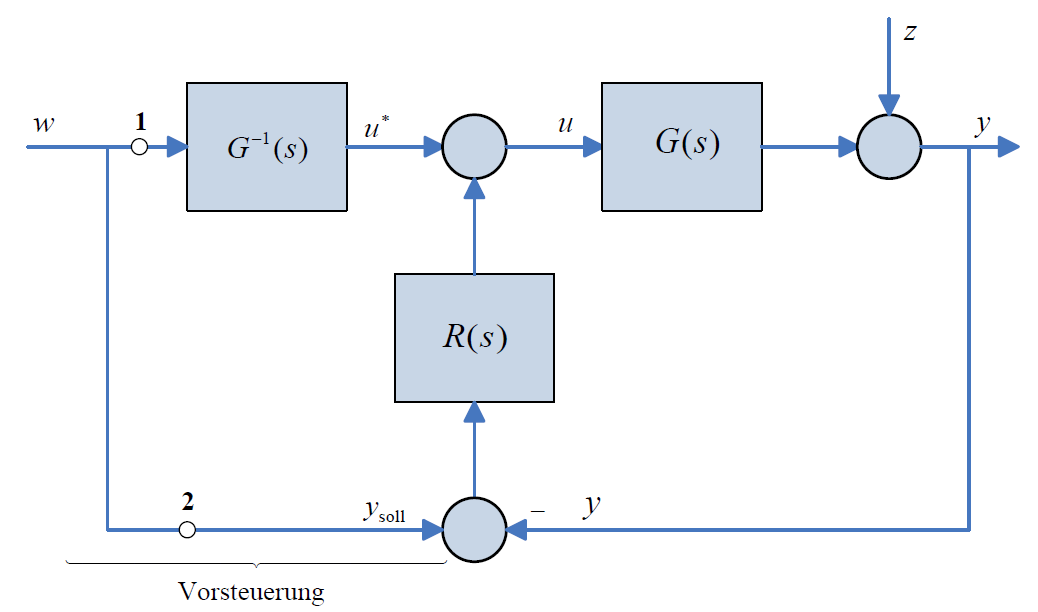
\includegraphics[width=0.5\columnwidth]{imgs/abb7_2.png}
\end{figure}

\textbf{Sonderfälle:}
\begin{itemize}
	\item Vorsteuerung ist nicht realisierbar (Zählergrad $>$ Nennergrad):
	\begin{itemize}
		\item Einfügen je eines PT$n$-Glieds bei $1$ und $2$ mit \\
		$V(s) = G_{PTn}(s) = \frac{1}{(1 + Ts)^n}$
		\item $n$ mindestens so groß wählen, dass $G^{-1}(s)G_{PTn}(s)$ realisierbar ist.
		\item[→] Führungsverhalten nicht mehr ideal
	\end{itemize}
	\item $G(s)$ besitzt eine rechts gelegene Nullstelle $\eta$:
	\begin{itemize}
		\item Einfügen je eines Glieds bei $1$ und $2$ mit \\
		$V(s) = \frac{1 - \frac 1 \eta s}{1 + Ts}$
	\end{itemize}
	\item  $G(s)$ enthält eine Totzeit $T_t$:
	\begin{itemize}
		\item Einfügen je eines Glieds bei $1$ und $2$ mit \\
		$V(s) = e^{-T_ts}$
	\end{itemize}
	\item Für alle Fälle gilt:
	\begin{itemize}
		\item $Y(s) = V(s) ⋅ W(s) + \frac{1}{1 + G(s) R(s)} Z(s)$
	\end{itemize}
	
\end{itemize}

\subsection{Störgrößenaufschaltung}
\begin{figure}[H]
	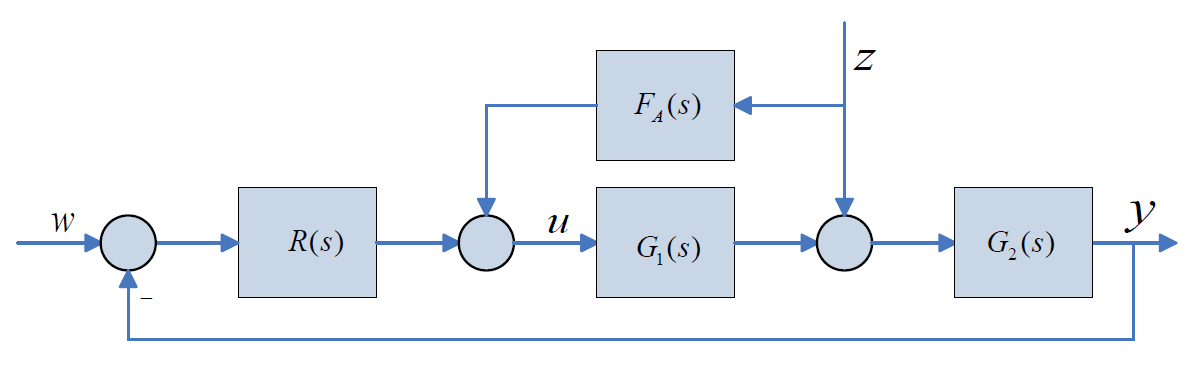
\includegraphics[width=0.7\columnwidth]{imgs/abb7_4.png}
\end{figure}

$$
	Y(s) = \frac{G_2(G_1 F_A + 1)}{1 + G_2 G_1 R} Z(s)
$$

\textbf{Ideale Störgrößenaufschaltung:}
$$
	F_A(s) = -\frac{1}{G_1(s)}, \tab \text{realisierbar, falls Zählergrad $<$ Nennergrad}
$$ ~\\

\textbf{Reale Störgrößenaufschaltung:}
$$
	F_A(s) = -\frac{1}{G_1(s)} ⋅ \underbrace{\frac{1}{(1 + Ts)^n}}_{\text{PTn-Glied}}
$$ ~\\

\textbf{Statische Störgrößenaufschaltung:}
$$
	F_A(s) = -\frac{1}{G_1(0)}
$$

\subsection{Kaskadenregelung}
\begin{figure}[H]
	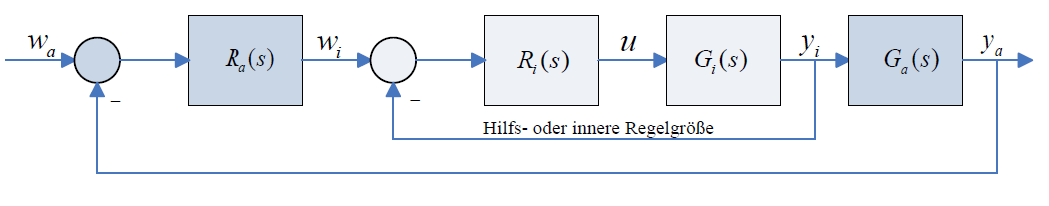
\includegraphics[width=0.8\columnwidth]{imgs/abb7_5.png}
\end{figure}

\textbf{Entwurf:}
\begin{enumerate}
	\item Entwurf eines Reglers $R_i(s)$ für die Regelstrecke $G_i(s)$, sodass ein günstiges Störverhalten von $y_i$ bei robuster Stabilität eintritt. \\
	Die Führungsübertragungsfunktion ist:
	$$
		T_i(s) = \frac{Y_i(s)}{W_i(s)} = \frac{G_i R_i}{1 + G_i R_i}
	$$
	\item Innere Schleife wird mit $G_a(s)$ zu der äußeren Schleife $\bar{G}_a(s) = T_i(s)G_a(s)$
	\item Entwurf eines Reglers $R_a(s)$ für die Regelstrecke $\bar G_a(s)$, sodass ein günstiges Störverhalten von $y_a$ mit zumeist stationärer Genauigkeit eintritt. \\
\end{enumerate}

\subsection{Zustandsregelung}
\subsubsection{Konstante Zustandsrückführung und Vorsteuerung}
\label{zustandsrueckfuehrung}
\begin{figure}[H]
	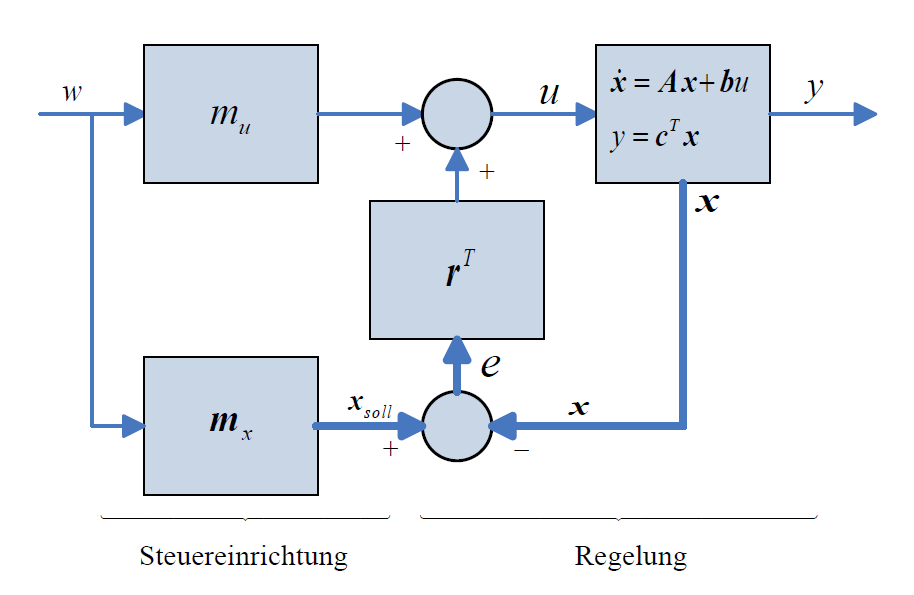
\includegraphics[width=0.7\columnwidth]{imgs/abb7_10.png}
\end{figure}

Sei die Strecke in Zustandsdarstellung mit $\dot x = Ax + bu$ und $y = c^T x$ \\

\textbf{Formeln}
$$
	\dot x(t) = (A - br^T)x + b(r^T m_x + m_u) w = A_r x + b_r w
$$
$$
	y(t) = c^Tx(t)
$$
$$
	u(t) = r^Te(t) + m_uw(t) = r^T(m_xw(t)-x(t)) + m_u w(t)
$$
$$
	G_{wy}(s) = T(s) = \frac{Y(s)}{W(s)} = c^T(sI-A_r)^{-1}b_r \tab (\text{Komplexe Übertragungsfunktion:})
$$ ~\\

\textbf{Variablen} ~\\
\begin{tabularx}{\columnwidth}{ll}
	\tab - & $A_r = (A - br^T)$ \\
	\tab - & $b_r = b(r^Tm_x + m_u)$ \\
\end{tabularx} ~\\

\textbf{Entwurf:} ~\\
$m_u, m_v$ bestimmen: ~\\
$$
	\vect{A & b \\ c^T & 0} ⋅ \vect{m_x \\ m_u} = \vect{0 \\ 1}
$$

$r^T$ bestimmen: ~\\
\begin{enumerate}
	\item Aufstellen des charakteristischen Polynoms (in Abh. von $r^T$ und $s$)$: \\
	\det(sI - A + br^T) = s^n + c_{n-1}(r_1, \dots, r_n) ⋅ s^{n-1} + \dots + c_0(r_1, \dots, r_n)$, \tab wobei $c_i = f(r_1, \dots, r_n)$
	\item Aufstellen eines Polynoms mit den gewünschten Eigenwerten (in Abh. von $s$): \\
	$P(s) = (s - p_1) ⋅ \dots ⋅ (s - p_n) = s^n + a_{n-1}s^{n - 1} + \dots + a_1s + a_0$, \tab wobei $p_i$ die gewünschten Eigenwerte sind
	\item Einsetzten der Variablen aus 1. und 2. in folgende Gleichungen und auflösen nach $r_1, \dots, r_n$: \\
	$$\begin{array}{c}
		c_{n-1}(r_1, \dots, r_n) = a_{n-1} \\
		\vdots \\
		c_0(r_1, \dots, r_n) = a_0
	\end{array}$$
\end{enumerate}

\subsubsection{Zustandsbeobachter}
\begin{figure}[H]
	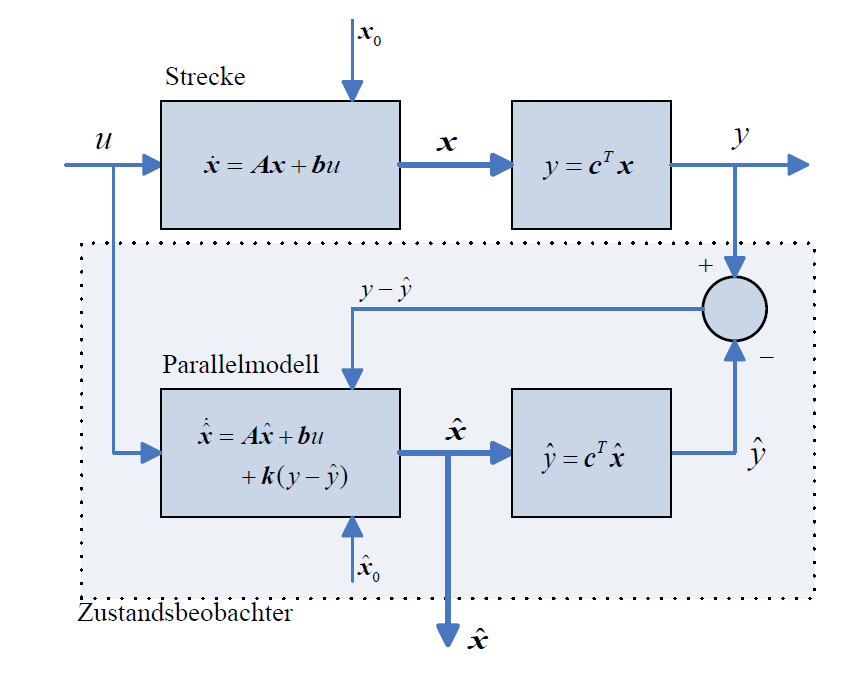
\includegraphics[width=0.7\columnwidth]{imgs/abb7_12.png}
\end{figure}

\textbf{Formeln:} ~\\
$
	\begin{array}{ll}
		\text{Zustandsschätzung} & \dot {\hat x} = A \hat x + bu + k(y - \hat y) = (A + kc^T)\hat x + bu + ky\\
		\text{Schätzung für }y & \hat y = c^T\hat x \\
		\text{Schätzfehler} & \tilde{x} = x - \hat x \\
		\text{Ableitung des Schätzfehlers} & \dot{\tilde x} = (A - kc^T)\tilde x = A_k \tilde x
	\end{array}
$ \\~\\

\textbf{Entwurf:}
\begin{enumerate}
	\item $\det(sI - A + kc^T) = s^n + c_{n-1}(k_1, \dots, k_n) ⋅ s^{n-1} + \dots + c_0(k_1, \dots, k_n)$, \tab wobei $c_i = f(k_1, \dots, k_n)$
	\item $P(s) = (s - p_1) ⋅ \dots ⋅ (s - p_n) = s^n + a_{n-1}s^{n - 1} + \dots + a_1s + a_0$, \tab wobei $p_i$ die gewünschten Eigenwerte sind
	\item Auflösen nach $k_1, \dots, k_n$: \\
	$$\begin{array}{c}
	c_{n-1}(k_1, \dots, k_n) = a_{n-1} \\
	\vdots \\
	c_0(k_1, \dots, k_n) = a_0
	\end{array}$$
\end{enumerate} ~\\

\subsection{Nichtlineare Zustandsregelung durch Ein-/Ausgangslinearisierung}

\textbf{Vorgehen:}
\begin{enumerate}
	\item Formulieren der nichtlinearen Streckenbeschreibung in der Zustandsdarstellung: \\
	$\dot x = a(x) + b(x) u$ \\
	$y = c(x) := c_0(x)$
	\item Ableiten von $y$ nach $x$ solange bis $u$ auftaucht: \\
	Wiederhole solange bis $b_q(x) ≠ 0$; starte mit $q = 1$; inkrementiere $q$ nach jedem Schritt um 1\\
	$y^{(q)} = \frac{\partial c_{q-1}}{\partial x_1} \dot x_1 + \dots + \frac{\partial c_{q-1}}{\partial x_n} \dot x_n = c_q(x) + b_q(x) u$
	\item Einsetzen von $y^{(i)} = c_i(x)$ in Wunschdifferentialgleichung \\
	$c_q(x) + b_q(x) u + a_{q-1} c_{q-1}(x) + \dots + a_0 c_0(x) = a_0 w$
	\item Auflösen nach $u$: \\
\end{enumerate}
Außerdem gilt:
$$
	Y(s) = \frac{a_0}{s^q + a_{q-1}s^{q-1} + \dots + a_0} W(s)
$$

\section{Digitale Realisierung}
\subsection{Tustin-Transformation}
Sei $z ⋅ u[k] = u[k + 1]$ sowie $z^{-1} ⋅ u[k] = u[k-1]$ \\
Die Tustin-Transformation ist definiert als:
\renewcommand{\arraystretch}{2}
$$
	\begin{array}{lll}
		R(z) = \frac{u[k]}{e[k]} = \frac{T(1+z^{-1})}{2(1 - z^{-1})} & \text{entspricht} & R(s) = \frac 1 s \\
		R(z) = \frac{u[k]}{e[k]} = \frac{2(1-z^{-1})}{T(1 + z^{-1})} & \text{entspricht} & R(s) = s \\	
	\end{array}
$$
\renewcommand{\arraystretch}{1.5}





\appendix

\pagebreak
\section{Mathematische Grundlagen}
\subsection{Partialbruchzerlegung}
\subsubsection{Partialbruchzerlegung mit Koeffizientenvergleich}
Sei $R(s) = \frac{b_ns^n + \dots + b_1s + b_0}{a_ms^m + \dots + a_1s + a_0}$ \\

1. Finde alle Polstellen $p_i$ von $R(s)$ \\

2. Setze Partialbrüche an: \\
$R(s) = G_1 + \dots + G_m = \frac{Z_1}{N_1} + \dots + \frac{Z_m}{N_m}, \tab G_i = \frac{Z_i}{N_i}$, wobei
\begin{itemize}
	\item $G_i = \frac{r_i}{s - p_i}$, für jeden einfachen reellen Pol $p_i$
	\item $G_i + G_{i+1} = \frac{r_i s + r_{i + 1}}{(s - p_i)(s - p_{i + 1})}$, für jedes konjugiert komplexes Polpaar $p_i, p_{i+1} = p_i^*$
	\item $G_i + \dots + G_k = \frac{r_i}{s - p_i} + \frac{r_{i+1}}{(s - p_i)^2} + \dots + \frac{r_{i + k - 1}}{(s - p_i)^k}$, für jeden k-fachen reellen Pol $p_i = p_{i+1} = \dots = p_{i + k - 1}$
\end{itemize}

3. Bringe alle Brüche auf denselben Nenner und addiere sie: \\
$R(s) = \frac{Z_1}{N_1} + \dots + \frac{Z_m}{N_m} = \frac{Z_1(N_2 + \dots + N_m)}{N_1 ⋅ \dots ⋅ N_n} + \dots + \frac{Z_m(N_1 + \dots + N_{m-1})}{N_1 ⋅ \dots ⋅ N_n} = \frac{Z_1(N_2 + \dots + N_m) + \dots + Z_m(N_1 + \dots + N_{m-1})}{N_1 ⋅ \dots ⋅ N_n}$ \\

4. Multipliziere den Zähler aus und forme um zu: \\
$ R(z) = \frac{(c_{1,m}r_1 + \dots + c_{m,m}r_m)s^m + \dots + (c_{1,0}r_1 + \dots + c_{m,0}r_m)s^0}{N_1 ⋅ \dots ⋅ N_n}$ \\

5. Löse folgendes lineare Gleichungssystem: \\
$\begin{array}{c}
(c_{1,m}r_1 + \dots + c_{m,m}r_m) = b_m \\
\vdots \\
(c_{1,0}r_1 + \dots + c_{m,0}r_m) = b_0
\end{array}$ \\

6. Setze $r_1$ bis $r_m$ in die Gleichung aus Schritt 2 ein ($R(s) = G_1 + \dots + G_m$) \\

%\subsubsection{Integration mit Partialbruchzerlegung}
%Sei $R(s) = \int \frac{b_ns^n + \dots + b_1s + b_0}{a_ms^m + \dots + a_1s + a_0} ~ds$ \\
%
%Befolge Schritt 1 - 6 \\
%
%$\implies R(s) = \int \frac{r_1}{s - p_1} + \dots + \frac{r_m}{s - s_l} + G_{l+1} + \dots + G_m ~ds$ \\
%$ = r_1\ln|s - p_1| + \dots + r_l\ln|s - p_l| + \int G_{l+1} + \dots + G_m ~ds$

\textbf{Beispiel:} ~\\
Sei $R(s) = \frac{5s-1}{s^2-1}$ \\

1. Finde alle Polstellen $p_i$ von $R(s):$ \\
$p_1 = -1$ und $p_2 = 1$ \\

2. Setze Partialbrüche an: \\
$\implies R(s) = \frac {r_1} {s - 1} + \frac {r_2} {s + 1}$ \\

3. Bringe alle Brüche auf denselben Nenner und addiere sie: \\
$R(s) = \frac{r_1(s + 1)}{s^2-1} + \frac{r_2(s - 1)}{s^2-1} = \frac{r_1(s + 1) + r_2(s - 1)}{s^2-1}$\\

4. Multipliziere den Zähler aus und forme um: \\
$ R(s) = \frac{(r_1 + r_2)s + (r_1 - r_2)}{s^2-1}$ \\

5. Löse folgendes lineare Gleichungssystem: \\
$r_1 + r_2 = 5$ \\
$r_1 - r_2 = -1$ \\
$\implies r_1 = 2 \land r_2 = 3$ \\

6. Setze $r_1$ und $r_2$ in die Gleichung aus Schritt 2 ein ($R(s) = \frac {r_1} {s - 1} + \frac {r_2} {s + 1}$): \\
$R(s) = \frac {2} {s - 1} + \frac {3} {s + 1}$

\subsubsection{Heavisidescher Zuhaltemethode}
Sei $R(s) = \frac{b_ns^n + \dots + b_1s + b_0}{a_ms^m + \dots + a_1s + a_0}$ \\

1. Finde alle Polstellen $p_i$ von $R(s)$ \\

2. Setze Partialbrüche an: \\
$R(s) = G_1 + \dots + G_m = \frac{Z_1}{N_1} + \dots + \frac{Z_m}{N_m}, \tab G_i = \frac{Z_i}{N_i}$, wobei
\begin{itemize}
	\item $G_i = \frac{r_i}{s - p_i}$, für jeden einfachen reellen Pol $p_i$
	\item $G_i + G_{i+1} = \frac{r_i}{(s - p_i)} + \frac{r_i^*}{(s - p_{i + 1})}$, für jedes konjugiert komplexes Polpaar $p_i, p_{i+1} = p_i^*$
	\item $G_i + \dots + G_k = \frac{r_i}{s - p_i} + \frac{r_{i+1}}{(s - p_i)^2} + \dots + \frac{r_{i + k - 1}}{(s - p_i)^k}$, für jeden k-fachen reellen Pol $p_i = p_{i+1} = \dots = p_{i + k - 1}$
\end{itemize}

3. Koeffizienten bestimmen: \\
$$
	r_i = \frac{b_ns^n + \dots + b_1s + b_0}{N_1 ⋅ \dots ⋅ N_{i-1} ⋅ N_{i+1} ⋅ \dots ⋅ N_{m}} \Bigg|_{s = p_i}
$$

4. Setze $r_1$ bis $r_m$ in die Gleichung aus Schritt 2 ein ($R(s) = G_1 + \dots + G_m$) \\

\subsection{Matrizen}
\subsubsection{Determinante}
\textbf{Determinante einer $2 \times 2$ Matrix} \\
Sei $A \in \mathbb{R}^{2 \times 2}$. \\
Die Determinante dieser Matrix ist definiert als:
$$
	\det(A) = |A| = a_{11}a_{22} - a_{21}a_{12}
$$

\subsubsection{Inverse}
\textbf{Inverse einer $2 \times 2$ Matrix} \\
Sei $A \in \mathbb{R}^{2 \times 2}$ und \\
sei $\det A ≠ 0$. \\
Die Inverse von A ist definiert als:
$$
	\frac{1}{\det A} ⋅ \vect{a_{22} & -a_{12} \\ -a_{21} & a_{11}}
$$

\section{Elektrotechnische Grundlagen}
\begin{tabular}{ll}
	Widerstand: & $U = R ⋅ I$ \\
	Kondensator: & $U = \frac{1}{C} \int I ~dt$, $I = C ⋅ \dot U$ \\
	Induktivität: & $U = L ⋅ \dot I$
\end{tabular}

\renewcommand{\arraystretch}{1}
\section{Physikalische Grundlagen}
\textbf{Masse-Feder-Dämpfer System}
\begin{figure}[H]
	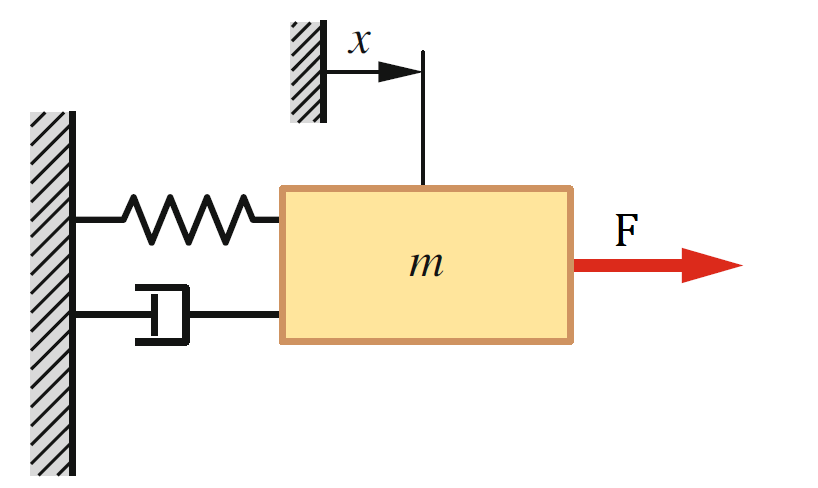
\includegraphics[width=0.3\columnwidth]{imgs/mass-spring-damper.png}
\end{figure}
$m$: Masse des Körpers, $d$: Dämpferkonstante, $k$: Federkonstante, $F$: Stellkraft
$$
	F = m ⋅ \ddot x + d \dot x + k x
$$

\renewcommand{\arraystretch}{1.5}



\pagebreak
\section*{Anmerkungen}
Dies ist eine Kurzzusammenfassung der Vorlesung Regelungstechnik an der Technischen Universität München.
Gehalten wurde diese Vorlesung durch Lohmann B. im Sommersemester 2019.
Ersteller dieser Zusammenfassung ist Gaida B.
Alle Angaben sind ohne Gewähr.


\section*{Literaturverzeichnis}
Werner Skolaut. \textit{Maschinenbau. Ein Lehrbuch für das ganze Bachelor-Studium}. Springer Vieweg. Heidelberg, 2018, S. 1271 - 1387





\end{document}

%TODO check for todos








